
%% bare_jrnl.tex
%% V1.3
%% 2007/01/11
%% by Michael Shell
%% see http://www.michaelshell.org/
%% for current contact information.
%%
%% This is a skeleton file demonstrating the use of IEEEtran.cls
%% (requires IEEEtran.cls version 1.7 or later) with an IEEE journal paper.
%%
%% Support sites:
%% http://www.michaelshell.org/tex/ieeetran/
%% http://www.ctan.org/tex-archive/macros/latex/contrib/IEEEtran/
%% and
%% http://www.ieee.org/



% *** Authors should verify (and, if needed, correct) their LaTeX system  ***
% *** with the testflow diagnostic prior to trusting their LaTeX platform ***
% *** with production work. IEEE's font choices can trigger bugs that do  ***
% *** not appear when using other class files.                            ***
% The testflow support page is at:
% http://www.michaelshell.org/tex/testflow/


%%*************************************************************************
%% Legal Notice:
%% This code is offered as-is without any warranty either expressed or
%% implied; without even the implied warranty of MERCHANTABILITY or
%% FITNESS FOR A PARTICULAR PURPOSE! 
%% User assumes all risk.
%% In no event shall IEEE or any contributor to this code be liable for
%% any damages or losses, including, but not limited to, incidental,
%% consequential, or any other damages, resulting from the use or misuse
%% of any information contained here.
%%
%% All comments are the opinions of their respective authors and are not
%% necessarily endorsed by the IEEE.
%%
%% This work is distributed under the LaTeX Project Public License (LPPL)
%% ( http://www.latex-project.org/ ) version 1.3, and may be freely used,
%% distributed and modified. A copy of the LPPL, version 1.3, is included
%% in the base LaTeX documentation of all distributions of LaTeX released
%% 2003/12/01 or later.
%% Retain all contribution notices and credits.
%% ** Modified files should be clearly indicated as such, including  *
%% ** renaming them and changing author support contact information. **
%%
%% File list of work: IEEEtran.cls, IEEEtran_HOWTO.pdf, bare_adv.tex,
%%                    bare_conf.tex, bare_jrnl.tex, bare_jrnl_compsoc.tex
%%*************************************************************************

% Note that the a4paper option is mainly intended so that authors in
% countries using A4 can easily print to A4 and see how their papers will
% look in print - the typesetting of the document will not typically be
% affected with changes in paper size (but the bottom and side margins will).
% Use the testflow package mentioned above to verify correct handling of
% both paper sizes by the user's LaTeX system.
%
% Also note that the "draftcls" or "draftclsnofoot", not "draft", option
% should be used if it is desired that the figures are to be displayed in
% draft mode.
%
\documentclass[journal]{IEEEtran}
%\documentclass{ieeeaccess}
%
% If IEEEtran.cls has not been installed into the LaTeX system files,
% manually specify the path to it like:
% \documentclass[journal]{../sty/IEEEtran}





% Some very useful LaTeX packages include:
% (uncomment the ones you want to load)


% *** MISC UTILITY PACKAGES ***
%
%\usepackage{ifpdf}
% Heiko Oberdiek's ifpdf.sty is very useful if you need conditional
% compilation based on whether the output is pdf or dvi.
% usage:
% \ifpdf
%   % pdf code
% \else
%   % dvi code
% \fi
% The latest version of ifpdf.sty can be obtained from:
% http://www.ctan.org/tex-archive/macros/latex/contrib/oberdiek/
% Also, note that IEEEtran.cls V1.7 and later provides a builtin
% \ifCLASSINFOpdf conditional that works the same way.
% When switching from latex to pdflatex and vice-versa, the compiler may
% have to be run twice to clear warning/error messages.






% *** CITATION PACKAGES ***
%
\usepackage{cite}
% cite.sty was written by Donald Arseneau
% V1.6 and later of IEEEtran pre-defines the format of the cite.sty package
% \cite{} output to follow that of IEEE. Loading the cite package will
% result in citation numbers being automatically sorted and properly
% "compressed/ranged". e.g., [1], [9], [2], [7], [5], [6] without using
% cite.sty will become [1], [2], [5]--[7], [9] using cite.sty. cite.sty's
% \cite will automatically add leading space, if needed. Use cite.sty's
% noadjust option (cite.sty V3.8 and later) if you want to turn this off.
% cite.sty is already installed on most LaTeX systems. Be sure and use
% version 4.0 (2003-05-27) and later if using hyperref.sty. cite.sty does
% not currently provide for hyperlinked citations.
% The latest version can be obtained at:
% http://www.ctan.org/tex-archive/macros/latex/contrib/cite/
% The documentation is contained in the cite.sty file itself.






% *** GRAPHICS RELATED PACKAGES ***
%
\ifCLASSINFOpdf
\usepackage[pdftex]{graphicx}
  % declare the path(s) where your graphic files are
  % \graphicspath{{../pdf/}{../jpeg/}}
  % and their extensions so you won't have to specify these with
  % every instance of \includegraphics
  % \DeclareGraphicsExtensions{.pdf,.jpeg,.png}
\else
  % or other class option (dvipsone, dvipdf, if not using dvips). graphicx
  % will default to the driver specified in the system graphics.cfg if no
  % driver is specified.
  % \usepackage[dvips]{graphicx}
  % declare the path(s) where your graphic files are
  % \graphicspath{{../eps/}}
  % and their extensions so you won't have to specify these with
  % every instance of \includegraphics
  % \DeclareGraphicsExtensions{.eps}
\fi
% graphicx was written by David Carlisle and Sebastian Rahtz. It is
% required if you want graphics, photos, etc. graphicx.sty is already
% installed on most LaTeX systems. The latest version and documentation can
% be obtained at: 
% http://www.ctan.org/tex-archive/macros/latex/required/graphics/
% Another good source of documentation is "Using Imported Graphics in
% LaTeX2e" by Keith Reckdahl which can be found as epslatex.ps or
% epslatex.pdf at: http://www.ctan.org/tex-archive/info/
%
% latex, and pdflatex in dvi mode, support graphics in encapsulated
% postscript (.eps) format. pdflatex in pdf mode supports graphics
% in .pdf, .jpeg, .png and .mps (metapost) formats. Users should ensure
% that all non-photo figures use a vector format (.eps, .pdf, .mps) and
% not a bitmapped formats (.jpeg, .png). IEEE frowns on bitmapped formats
% which can result in "jaggedy"/blurry rendering of lines and letters as
% well as large increases in file sizes.
%
% You can find documentation about the pdfTeX application at:
% http://www.tug.org/applications/pdftex


\usepackage{epstopdf}


% *** MATH PACKAGES ***
%
\usepackage[cmex10]{amsmath}
% A popular package from the American Mathematical Society that provides
% many useful and powerful commands for dealing with mathematics. If using
% it, be sure to load this package with the cmex10 option to ensure that
% only type 1 fonts will utilized at all point sizes. Without this option,
% it is possible that some math symbols, particularly those within
% footnotes, will be rendered in bitmap form which will result in a
% document that can not be IEEE Xplore compliant!
%
% Also, note that the amsmath package sets \interdisplaylinepenalty to 10000
% thus preventing page breaks from occurring within multiline equations. Use:
%\interdisplaylinepenalty=2500
% after loading amsmath to restore such page breaks as IEEEtran.cls normally
% does. amsmath.sty is already installed on most LaTeX systems. The latest
% version and documentation can be obtained at:
% http://www.ctan.org/tex-archive/macros/latex/required/amslatex/math/





% *** SPECIALIZED LIST PACKAGES ***
%
%\usepackage{algorithmic}
% algorithmic.sty was written by Peter Williams and Rogerio Brito.
% This package provides an algorithmic environment fo describing algorithms.
% You can use the algorithmic environment in-text or within a figure
% environment to provide for a floating algorithm. Do NOT use the algorithm
% floating environment provided by algorithm.sty (by the same authors) or
% algorithm2e.sty (by Christophe Fiorio) as IEEE does not use dedicated
% algorithm float types and packages that provide these will not provide
% correct IEEE style captions. The latest version and documentation of
% algorithmic.sty can be obtained at:
% http://www.ctan.org/tex-archive/macros/latex/contrib/algorithms/
% There is also a support site at:
% http://algorithms.berlios.de/index.html
% Also of interest may be the (relatively newer and more customizable)
% algorithmicx.sty package by Szasz Janos:
% http://www.ctan.org/tex-archive/macros/latex/contrib/algorithmicx/




% *** ALIGNMENT PACKAGES ***
%
%\usepackage{array}
% Frank Mittelbach's and David Carlisle's array.sty patches and improves
% the standard LaTeX2e array and tabular environments to provide better
% appearance and additional user controls. As the default LaTeX2e table
% generation code is lacking to the point of almost being broken with
% respect to the quality of the end results, all users are strongly
% advised to use an enhanced (at the very least that provided by array.sty)
% set of table tools. array.sty is already installed on most systems. The
% latest version and documentation can be obtained at:
% http://www.ctan.org/tex-archive/macros/latex/required/tools/


\usepackage{mdwmath}
\usepackage{mdwtab}
% Also highly recommended is Mark Wooding's extremely powerful MDW tools,
% especially mdwmath.sty and mdwtab.sty which are used to format equations
% and tables, respectively. The MDWtools set is already installed on most
% LaTeX systems. The lastest version and documentation is available at:
% http://www.ctan.org/tex-archive/macros/latex/contrib/mdwtools/


% IEEEtran contains the IEEEeqnarray family of commands that can be used to
% generate multiline equations as well as matrices, tables, etc., of high
% quality.


%\usepackage{eqparbox}
% Also of notable interest is Scott Pakin's eqparbox package for creating
% (automatically sized) equal width boxes - aka "natural width parboxes".
% Available at:
% http://www.ctan.org/tex-archive/macros/latex/contrib/eqparbox/





% *** SUBFIGURE PACKAGES ***
\usepackage[tight,footnotesize]{subfigure}
% subfigure.sty was written by Steven Douglas Cochran. This package makes it
% easy to put subfigures in your figures. e.g., "Figure 1a and 1b". For IEEE
% work, it is a good idea to load it with the tight package option to reduce
% the amount of white space around the subfigures. subfigure.sty is already
% installed on most LaTeX systems. The latest version and documentation can
% be obtained at:
% http://www.ctan.org/tex-archive/obsolete/macros/latex/contrib/subfigure/
% subfigure.sty has been superceeded by subfig.sty.



%\usepackage[caption=false]{caption}
%\usepackage[font=footnotesize]{subfig}
% subfig.sty, also written by Steven Douglas Cochran, is the modern
% replacement for subfigure.sty. However, subfig.sty requires and
% automatically loads Axel Sommerfeldt's caption.sty which will override
% IEEEtran.cls handling of captions and this will result in nonIEEE style
% figure/table captions. To prevent this problem, be sure and preload
% caption.sty with its "caption=false" package option. This is will preserve
% IEEEtran.cls handing of captions. Version 1.3 (2005/06/28) and later 
% (recommended due to many improvements over 1.2) of subfig.sty supports
% the caption=false option directly:
%\usepackage[caption=false,font=footnotesize]{subfig}
%
% The latest version and documentation can be obtained at:
% http://www.ctan.org/tex-archive/macros/latex/contrib/subfig/
% The latest version and documentation of caption.sty can be obtained at:
% http://www.ctan.org/tex-archive/macros/latex/contrib/caption/




% *** FLOAT PACKAGES ***
%
%\usepackage{fixltx2e}
% fixltx2e, the successor to the earlier fix2col.sty, was written by
% Frank Mittelbach and David Carlisle. This package corrects a few problems
% in the LaTeX2e kernel, the most notable of which is that in current
% LaTeX2e releases, the ordering of single and double column floats is not
% guaranteed to be preserved. Thus, an unpatched LaTeX2e can allow a
% single column figure to be placed prior to an earlier double column
% figure. The latest version and documentation can be found at:
% http://www.ctan.org/tex-archive/macros/latex/base/



%\usepackage{stfloats}
% stfloats.sty was written by Sigitas Tolusis. This package gives LaTeX2e
% the ability to do double column floats at the bottom of the page as well
% as the top. (e.g., "\begin{figure*}[!b]" is not normally possible in
% LaTeX2e). It also provides a command:
%\fnbelowfloat
% to enable the placement of footnotes below bottom floats (the standard
% LaTeX2e kernel puts them above bottom floats). This is an invasive package
% which rewrites many portions of the LaTeX2e float routines. It may not work
% with other packages that modify the LaTeX2e float routines. The latest
% version and documentation can be obtained at:
% http://www.ctan.org/tex-archive/macros/latex/contrib/sttools/
% Documentation is contained in the stfloats.sty comments as well as in the
% presfull.pdf file. Do not use the stfloats baselinefloat ability as IEEE
% does not allow \baselineskip to stretch. Authors submitting work to the
% IEEE should note that IEEE rarely uses double column equations and
% that authors should try to avoid such use. Do not be tempted to use the
% cuted.sty or midfloat.sty packages (also by Sigitas Tolusis) as IEEE does
% not format its papers in such ways.


%\ifCLASSOPTIONcaptionsoff
%  \usepackage[nomarkers]{endfloat}
% \let\MYoriglatexcaption\caption
% \renewcommand{\caption}[2][\relax]{\MYoriglatexcaption[#2]{#2}}
%\fi
% endfloat.sty was written by James Darrell McCauley and Jeff Goldberg.
% This package may be useful when used in conjunction with IEEEtran.cls'
% captionsoff option. Some IEEE journals/societies require that submissions
% have lists of figures/tables at the end of the paper and that
% figures/tables without any captions are placed on a page by themselves at
% the end of the document. If needed, the draftcls IEEEtran class option or
% \CLASSINPUTbaselinestretch interface can be used to increase the line
% spacing as well. Be sure and use the nomarkers option of endfloat to
% prevent endfloat from "marking" where the figures would have been placed
% in the text. The two hack lines of code above are a slight modification of
% that suggested by in the endfloat docs (section 8.3.1) to ensure that
% the full captions always appear in the list of figures/tables - even if
% the user used the short optional argument of \caption[]{}.
% IEEE papers do not typically make use of \caption[]'s optional argument,
% so this should not be an issue. A similar trick can be used to disable
% captions of packages such as subfig.sty that lack options to turn off
% the subcaptions:
% For subfig.sty:
% \let\MYorigsubfloat\subfloat
% \renewcommand{\subfloat}[2][\relax]{\MYorigsubfloat[]{#2}}
% For subfigure.sty:
% \let\MYorigsubfigure\subfigure
% \renewcommand{\subfigure}[2][\relax]{\MYorigsubfigure[]{#2}}
% However, the above trick will not work if both optional arguments of
% the \subfloat/subfig command are used. Furthermore, there needs to be a
% description of each subfigure *somewhere* and endfloat does not add
% subfigure captions to its list of figures. Thus, the best approach is to
% avoid the use of subfigure captions (many IEEE journals avoid them anyway)
% and instead reference/explain all the subfigures within the main caption.
% The latest version of endfloat.sty and its documentation can obtained at:
% http://www.ctan.org/tex-archive/macros/latex/contrib/endfloat/
%
% The IEEEtran \ifCLASSOPTIONcaptionsoff conditional can also be used
% later in the document, say, to conditionally put the References on a 
% page by themselves.





% *** PDF, URL AND HYPERLINK PACKAGES ***
%
\usepackage{url}
% url.sty was written by Donald Arseneau. It provides better support for
% handling and breaking URLs. url.sty is already installed on most LaTeX
% systems. The latest version can be obtained at:
% http://www.ctan.org/tex-archive/macros/latex/contrib/misc/
% Read the url.sty source comments for usage information. Basically,
% \url{my_url_here}.

%-----------------Custom packages ----------------------------------
\usepackage{color}
\usepackage{mathtools}
%----------------End Custom Packages------------------------------


% *** Do not adjust lengths that control margins, column widths, etc. ***
% *** Do not use packages that alter fonts (such as pslatex).         ***
% There should be no need to do such things with IEEEtran.cls V1.6 and later.
% (Unless specifically asked to do so by the journal or conference you plan
% to submit to, of course. )


% correct bad hyphenation here
\hyphenation{op-tical net-works semi-conduc-tor}


\begin{document}
%
% paper title
% can use linebreaks \\ within to get better formatting as desired
\title{Experimental Testing of a Real-Time Implementation of a PMU-based Wide-Area Damping Control System}
%
%
% author names and IEEE memberships
% note positions of commas and nonbreaking spaces ( ~ ) LaTeX will not break
% a structure at a ~ so this keeps an author's name from being broken across
% two lines.
% use \thanks{} to gain access to the first footnote area
% a separate \thanks must be used for each paragraph as LaTeX2e's \thanks
% was not built to handle multiple paragraphs
%

%%Fix Later : Move Luigi as first author.

\author{Eldrich~Rebello, Luigi~Vanfretti~\IEEEmembership{Senior~Member,~IEEE}, Muhammad~Shoaib~Almas,~\IEEEmembership{Member, IEEE}
                % <-this % stops a space
\thanks{Eldrich Rebello is currently with the Wind Energy Institute of Canada
e-mail:  \mbox{eldrich.rebello@alumni.aalto.fi}}% <-this % stops a space
\thanks{M. Shoaib Almas is with KTH Royal Institute of Technology, Stockholm, Sweden. email: msalmas@kth.se}% <-this % stops a space
\thanks{Luigi Vanfretti is an associate Professor at Rensselaer Polytechnic Institute  email : vanfrl@rpi.edu}}

% note the % following the last \IEEEmembership and also \thanks - 
% these prevent an unwanted space from occurring between the last author name
% and the end of the author line. i.e., if you had this:
% 
% \author{....lastname \thanks{...} \thanks{...} }
%                     ^------------^------------^----Do not want these spaces!
%
% a space would be appended to the last name and could cause every name on that
% line to be shifted left slightly. This is one of those "LaTeX things". For
% instance, "\textbf{A} \textbf{B}" will typeset as "A B" not "AB". To get
% "AB" then you have to do: "\textbf{A}\textbf{B}"
% \thanks is no different in this regard, so shield the last } of each \thanks
% that ends a line with a % and do not let a space in before the next \thanks.
% Spaces after \IEEEmembership other than the last one are OK (and needed) as
% you are supposed to have spaces between the names. For what it is worth,
% this is a minor point as most people would not even notice if the said evil
% space somehow managed to creep in.



% The paper headers
\markboth{Journal Title}%
{Shell \MakeLowercase{\textit{et al.}}: Bare Demo of IEEEtran.cls for Journals}
% The only time the second header will appear is for the odd numbered pages
% after the title page when using the twoside option.
% 
% *** Note that you probably will NOT want to include the author's ***
% *** name in the headers of peer review papers.                   ***
% You can use \ifCLASSOPTIONpeerreview for conditional compilation here if
% you desire.




% If you want to put a publisher's ID mark on the page you can do it like
% this:
%\IEEEpubid{0000--0000/00\$00.00~\copyright~2007 IEEE}
% Remember, if you use this you must call \IEEEpubidadjcol in the second
% column for its text to clear the IEEEpubid mark.



% use for special paper notices
%\IEEEspecialpapernotice{(Invited Paper)}




% make the title area
\maketitle


\begin{abstract}
%\boldmath
The modern power grid is increasingly being used under operating conditions of increasing stress, giving rise to grid stability issues. One of these stability issues is the phenomenon of inter-area oscillations. Simulations have demonstrated the advantages of Wide-area Measurement Signals (WAMS)-based Oscillation Damping Controls in achieving improved electromechanical mode damping compared to traditional, local signal-based Power System Stabilizers (PSS). This work takes an existing Phasor-based oscillation damping (POD) algorithm and uses it to implement a proof-of-concept, real-time controller on National Instruments hardware. The developed prototype is tested in a real-time Hardware-in-the-loop setup (RT-HIL) using OPAL-RT\rq{s} e\textsc{megasim} real-time simulation platform and synchrophasor data from actual Phasor Measurement Units (PMUs). The prototype and experiments provide insight into the feasibility and real-world limitations of wide-area controls. Further, it is demonstrated how the proposed control architecture has applications independent of the controlled device. Challenges faced, the solutions implemented together with the present prototype\rq{s} limitations are also discussed.

%Version 0.32 Abstract

%The modern power grid is increasingly being used under operating conditions of increasing stress for which it was not designed, giving rise to grid stability issues. One of these stability issues is the phenomenon of low frequency, electro-mechanically induced, inter-area oscillations. Simulations have demonstrated the potential of Wide Area Measurement Signals (WAMS)-based Power Oscillation Damping (POD) in achieving improved electromechanical mode damping compared to traditional, local signal based, Power System Stabilizers (PSS). \iffalse Also, the adoption of synchrophasor measurement data from Phasor Measurement Units (PMU's) is rising annually.\fi This paper takes an established Phasor-based oscillation damping algorithm and combines it with modern PMU technology to implement a hardware prototype of a real-time oscillation damping control system using remote PMU signals sent over a communications network. The developed prototype is tested in real-time using a Hardware-in-the-loop approach in conjunction with the Klein-Rogers-Kundur two-area four-machine test system and is demonstrated to have applications independent of the controlled device.

%The developed hardware prototype has been tested using Real-Time hardware-in-the-loop (HIL) approach and the simulations are performed on Klien-Roger-Kundur two area four machine test system. 

\end{abstract}

% Note that keywords are not normally used for peerreview papers.
\begin{IEEEkeywords}
WAPOD, WAMPAC, synchrophasor, PMU, damping control, Wide Area measurement and control
\end{IEEEkeywords}






% For peer review papers, you can put extra information on the cover
% page as needed:
% \ifCLASSOPTIONpeerreview
% \begin{center} \bfseries EDICS Category: 3-BBND \end{center}
% \fi
%
% For peerreview papers, this IEEEtran command inserts a page break and
% creates the second title. It will be ignored for other modes.
\IEEEpeerreviewmaketitle



\section{Introduction}
\IEEEPARstart{A}{lthough} the purpose of interconnecting disparate power networks was to increase stability, the present situation of the power system incorporates renewable energy sources and power trading corridors, both of which impact system stability. One of these stability issues is the phenomenon of inter- and intra-area electromechanical oscillations\cite{KundurTwoArea}. Inter-area oscillations involve groups of generators oscillating against each other and these groups are typically connected by weak tie-lines\cite{KundurTwoArea}. Inter-area oscillations are of a lower frequency ($<1 Hz$) relative to intra-area oscillations and are often poorly damped leading to stability problems\cite{KundurTwoArea}. Modern solutions to the problems of inter-area and intra-area oscillations use Power System Stabilizers (PSS) \cite{WAPODNorway}. While a PSS provides excellent damping to intra-area modes with good local observability, its performance with inter-area modes may not be satisfactory \cite{localREMcomparison}. The limited observability in a local signal can be complemented by wide-area, synchrophasor data. Wide-area data allows for calculations and observations such as voltage angle differences, which are not possible with solely local measurement data\cite{Yuwa}. For a more complete treatment of the phenomenon of power system oscillations, see \cite{Rogers_book}.
%\subsection{Motivation}
\vspace{-1em}

\subsection{Literature Review}

\subsubsection*{Analytical Studies}

It has been shown in \cite{Yuwa} that wide-area signals are preferable to local signals, such as active power and frequency, \cite{localREMcomparison} for the purpose of damping inter-area oscillations. Studies such as \cite{Yuwa} have analysed damping performance when using signals such as voltage angle difference, which can easily be computed using data from multiple PMUs.

\subsubsection*{Field Tests}
Successful field trials of wide-area oscillation damping controllers are reported in \cite{WAPODNorway} and \cite{WAPODChina} indicating the potential that PMU-based wide area controllers have to offer. These results are not without certain limitations. In \cite{WAPODNorway} it is reported that the limited set of tests conducted with the Wide Area Power Oscillation Damper (WAPOD) are insufficient to compare the performance of a WAPOD to a local-measurement based controller. Coordinating field experiments is often difficult and requires the participation of several entities. This work attempts to approximate real-world conditions as closely as possible but avoids several of the limitations of working with an operational power system.

\subsubsection*{Delay Studies} The damping performance of a controller that depends on TCP network-transmitted data for input is constrained by the network transport delay. Beyond a certain value of time delay, damping will cease to be effective. These effects are explored in more detail in \cite{China_paper} and \cite{Biplab}.\vspace{-1em}

\subsection{Paper Contributions}
The goal of this paper is to imlement a hardware prototype and to demonstrate experimentally the potential and flexibility in oscillation damping controller design that is possible by using synchrophasor data (IEEE C37.118). The Phasor Power Oscillation Damping (Phasor-POD) algorithm originally developed by \"{A}ngquist and Gama\cite{PhasorPOD} is implemented and deployed on a National Instruments Compact Reconfigurable Input / Output (cRIO) real-time controller. A modified, \textsc{Simulink} model of the four-machine, two-area network developed by Klein-Rogers and Kundur \cite{KundurTwoArea} is executed in real-time on the eMEGASIM \cite{eMEGASIM} platform from OPAL-RT. \iffalse This allows interfacing an externally generated control signal with the simulated model in real-time.\fi A Hardware-in-the-loop (HIL) test is set up to verify the performance of the hardware implementation of the Phasor POD algorithm. The flexibility of the developed controller is also demonstrated by extracting various data from the synchrophasor data-set and using each as a damping input to the controller. This paper also illustrates that the controller can have multiple applications by testing it with two different controllable devices; a generator automatic voltage regulator (AVR) system and a Flexible AC Transmission System (FACTS)-device excitation system. A brief analysis of the performance of each synchrophasor input to the hardware POD is also presented.\\\vspace{-1em}

In the context of this paper, the term `\emph{real-time}' is used to refer to a controller where input data is processed and made available as output within a deterministic time frame. The usage of the term is similar to that in the field of embedded systems in that strict deadlines are imposed and system reaction time is guaranteed and fixed. To this end, the real-time simulator's clock runs as fast as an actual clock and therefore generates and processes data in real-time. This requires that any external, hardware controllers connected to it operate at an identical pace. These constraints imply that the algorithm implementation in this work is tested under conditions that closely approximate a real-world situation. Constraints such as signal magnitude limits, variable network communication delays and noise apply. If the proposed hardware implementation of the POD algorithm fails to respond in a deterministic manner, it is deemed to have failed.\\\vspace{-1em}

Problems exist with traditional damping controller design that is based around model linearisation and non-linear simulations \cite{WAPODChina}. This paper circumvents these issues by adopting a phasor-based damping algorithm \cite{PhasorPOD} that can operate independent of the network configuration. In addition, beacuse this is the same algorithm used in proprietary implementations\cite{WAPODNorway}, the prototype developed is directly comparable to other real-world implementations. The developed controller is designed with modularity and portability in mind and is demonstrated to be able to provide effective damping in multiple application scenarios. Although \cite{Yuwa} presents a scenario where the generator AVR\rq{s} error signal is modulated using PMU data, this work presents an experimental validation of those results. While multi-mode damping can be attractive \cite{Kamwa}, the focus of this work is  single-mode damping to verify and be comparble to real-world cases \cite{WAPODNorway}, \cite{WAPODChina} .

\subsection{Paper Organisation}

This paper is organised as follows. Section \ref{Background} presents a brief, theoretical background of the work presented in this study while Section \ref{softhardware} introduces the software and hardware used. Section \ref{SetupPreparation} covers the preparation of the \textsc{Simulink} models for real-time simulation and two real-time test cases, one with the WAPOD input fed to the excitation system of a Static VAR Compensator (SVC) and the other with the WAPOD modulating the input of a generator\rq{s} Automatic Voltage Regulator (AVR). The results obtained from the two tests are presented and analysed in Section \ref{Results}. Section \ref{Challenges} examines some of the major challenges faced in the development, implementation and testing of this WAPOD controller. No experimental implementation is ever ready for the field and there is always room for improvement. This is outlined in Section \ref{Future} and finally conclusions are drawn in Section \ref{Conclusion}.
%---------------------------------------------------------------------------------------------------------------------------------------------------
\section{Background}\label{Background}

%As modern power systems grow in size, both in terms of power transfer capacity and geographic spread, they are increasingly being used for purposes that they were not designed for. Examples of these \textquoteleft new\textquoteright ~uses include conditions of increasing stress such as power trading between countries. These interconnections, which link synchronous generators, often separated by vast physical distances, create conditions where small disturbances can excite oscillations that may or may not settle. When the generators of one area oscillate at a low frequency (typically 0.2\textendash 2.5Hz) against the generators of another interconnected, but distinct area, \textquoteleft inter-area\textquoteright ~oscillations may be excited.

%Although the purpose of system interconnection was to increase stability, the present situation of the power system incorporates renewable energy sources and power trading corridors, both of which impact system stability. More modern solutions to the problems of inter area and intra oscillations use Power System Stabilizers (PSS) \cite{Dmello}. While a PSS provides excellent damping to intra area modes with good local observability, its performance with inter-area modes may not be satisfactory \cite{localREMcomparison}.\\
% needed in second column of first page if using \IEEEpubid
%\IEEEpubidadjcol
%\subsection{Previous Experiences}
\subsection{Why the phasor-based algorithm?}  %one word missing between controller and choice. could be topology or design?
Traditional controllers for FACTS devices depend on accurate system models at a specific operating condition. Large systems often experience changes in their topology and data about the present condition may not always be available to apply conventional control design methods. Further, identifying system oscillation modes and designing appropriate dampers is based on small signal and linear analysis techniques applied to power system models. These models are often difficult to derive accurately for large and inter-connected power systems \cite{WAMTCSC}. Linearised models are also only valid for small deviations from the linearisation point. One important reason for choosing the Phasor-POD algorithm for real-time implementation in this work was the fact that the algorithm itself uses limited inputs and is independent of network configuration and topology. The only network-dependent algorithm parameter is the oscillation frequency and this is usually known from system studies or can be determined directly from synchrophasor measurements \cite{TaskForce}. Compared to conventional controllers designed using linearisation-based methods, the adoption of phasor-based controllers has not been common mainly due to the fact that such controllers tend to be highly non-linear and thus difficult to, both, model in simulation studies \cite{Chaudhuri} and implement in real-time applications \cite{WAPODNorway}.

\subsection{Phasor POD Algorithm}

Some of the problems that emerge from the model linearisation approach are addressed by phasor-based oscillation damping algorithms. The algorithm chosen for implementation here is the Phasor-POD algorithm developed by \"{A}ngquist and Gama\cite{PhasorPOD}. The measured signal can be represented as a space-phasor \cite{Chaudhuri}: 

\begin{equation}
%\begin{multlined}
s(t)={s}_{avg}+\mathrm{Re}\left\{{\stackrel{\to }{s}}_{ph}\cdot {e}^{{jwt}}\right\}
%\mbox{where, } {\stackrel{\to }{s}}_{ph} \mbox{ is a complex phasor, rotating at the frequency }\\ \omega
%\end{multlined}
\end{equation}
%equation goes here!!

\noindent{where}, $\stackrel{\to }{s}_{ph}$ is a complex phasor, rotating at the frequency $\omega$ \cite{PhasorPOD}. This presents an average value and the associated oscillatory part, in a stationary reference frame. The oscillating part can then be used to generate a control signal for the FACTS (or other controllable device) using a control algorithm. This method is independent of the system state or configuration and is not computationally intensive. Controllers based on this approach may also incorporate error checking and phasor estimation algorithms. The real-time hardware implementation of the Phasor-POD algorithm was based on the \textsc{Simulink} implementation in \cite{PhasorPODImplement} and its goal was to replicate the behaviour of the \textsc{Simulink} implementation as closely as possible. The algorithm accepts three inputs; the search frequency, $\omega_{cs1}$, the sampling time $T_{s}$, the phase correction $alpha$ in addition to a signal scaling factor. It takes advantage of the fact that the oscillation frequency for a given network configuration is usually known, which in this case is the 0.64Hz inter-area mode. Using this known frequency value, a  co-ordinate system, rotating at this known frequency, is set up where the oscillating component is continuously extracted as a phasor \cite{PhasorPOD}. In simpler terms, the Phasor-POD algorithm separates an input signal into an average valued and an oscillating component. The oscillating component, when suitably phase-shifted, can be used as a supplementary damping input to a generator's AVR or the excitation system of a FACTS device.
%\begin{equation} \label{phasoreqn}
%\left(t\right)={s}_{avg}+\mathrm{Re}\left\{{\stackrel{\to }{s}}_{ph}\cdot {e}^{{j}^{wt}}\right\} \cite{Chaudhuri}
%\end{equation}
%\begin{figure}[!h]
%\centering
%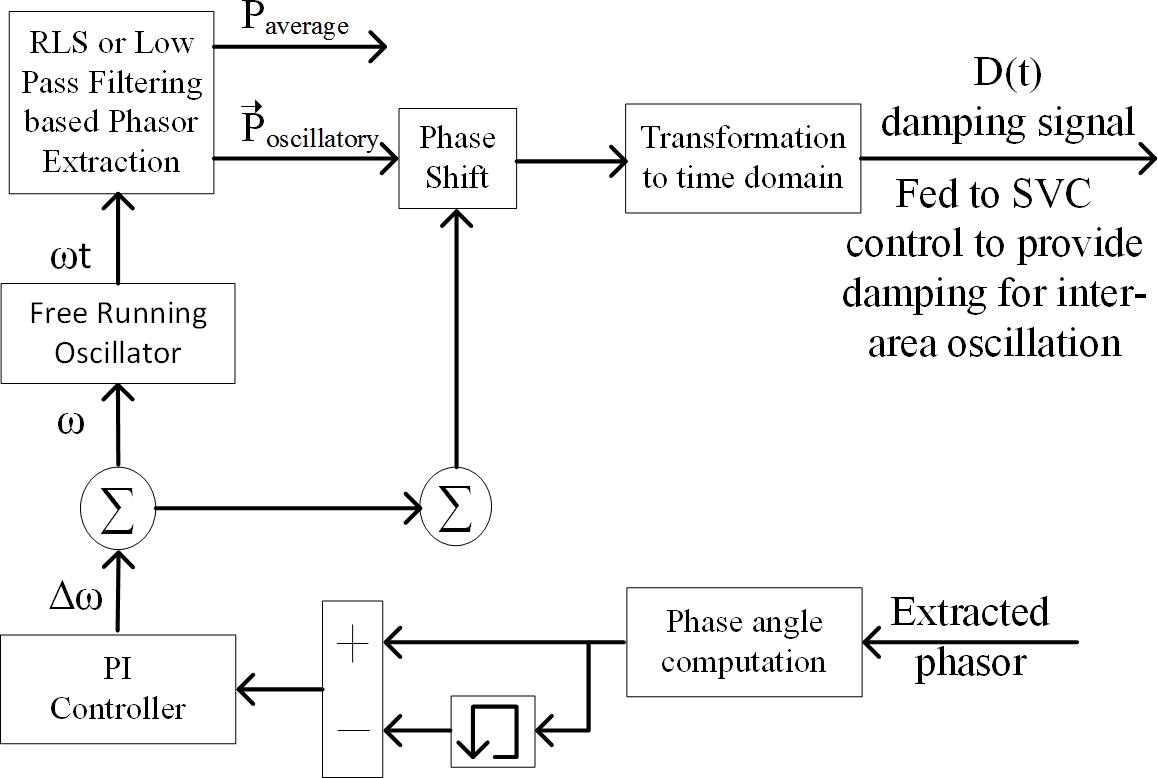
\includegraphics[width=3.5in]{PhasorPODAlgorithm.png} 
%\caption{Phasor-POD Block Diagram}
%\label{PhasorPODDiagram}
%\end{figure}
%-----------------------------------------------------------------------------------------------------------------------------------------------
\section{Software Architecture and Hardware Configuration}\label{softhardware}

The WAPOD\footnote{Historically, damping stabilizers have been termed WAPOD where the P represents a measurement of active power through the line. Active power here would be used as a controller input signal. Although this term is not accurate when other quantities are used as control inputs or feedback signals, the term is used here to maintain consistency with existing literature.} prototype developed here uses commercially available micro-controller hardware and uses PMU measurements received over a TCP/IP network. The Phasor-POD algorithm \cite{PhasorPOD} was executed on the control hardware in real-time. The inputs to the controller come from one or multiple PMU's, each monitoring data at different points of the power system. The power system model used in this paper is the two-area four-machine model, originally proposed by Klein, Rogers and Kundur \cite{KundurTwoArea}. To prove the real-world applicability of the developed controller, all tests are carried out in real-time, with conditions such as measurement noise and communication network delay present.

\subsection{Hardware Configuration}
The power system model was simulated in real-time on OPAL-RT's e\textsc{Megasim} \cite{eMEGASIM} real-time simulation platform (Figure \ref {Hardware_Outline}). This model was interfaced with externally generated, analogue signals in a HIL configuration. Current and voltage signals from different points (Buses 5 and 11 in Figure \ref{NetworkOutline}) on the simulated network are extracted as analogue signals, amplified and then supplied as inputs to two PMUs. Two cRIO-9076 \cite{cRIO9081} devices are used as PMUs, although any other commercial device could be used. Each PMU is equipped with three-phase analogue voltage and current input modules in addition to GPS time synchronisation. The PMUs report data every 20 ms. The synchrophasor data stream  generated by these PMUs is sent over a TCP/IP network to a Phasor Data Concentrator (PDC) which produces a time-aligned output stream. This stream is then accessed on a PC running LabVIEW over a TCP/IP network. Data is extracted and sent to the FPGA (Field Programmable Gate Array) running the Phasor-POD algorithm. The FPGA on the cRIO-9081 \cite{cRIO9081} generates a damping signal which is then wired back to the real-time simulator for use in the \textsc{Simulink} model.

\begin{figure}[htpb]
\centering
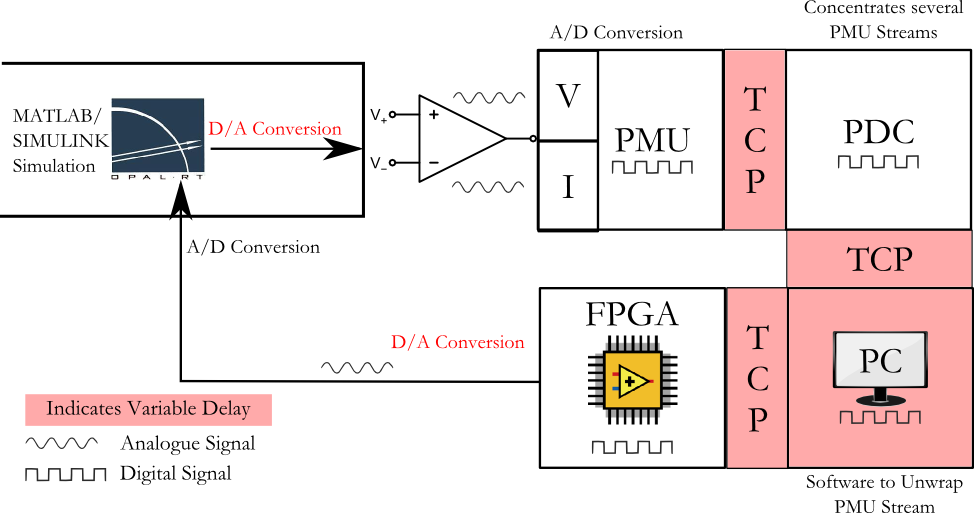
\includegraphics[width=3.5in]{DataFlow.png} 
\caption{Hardware loop showing complete data path, signal nature at each point and sources of delay}
\label{Hardware_Outline}
\vspace{-1em}
\end{figure}
%\vspace{-0.5em}

\cite{PhasorPODImplement} describes the details of the equipment used here. It is important to note that the data flow in Figure~\ref{Hardware_Outline} involves both D/A and A/D conversions. Also, because no synchronisation is used for these conversions, it is important that the sample rates or loop rates of each section be integer multiples of each other. This prevents data sampling errors. The issue of different loop rates is discussed in Section \ref{looprate}.

%An image of the physical setup is included for clarity in Appendix \ref{SetupImage}. 

\subsection{Software Architecture}
%The two-area four-machine model used here is available in \textsc{Simulink}'s SimPowerSystems. The \textsc{Simulink} implementation of the Phasor-POD algorithm was developed by Almas and Vanfretti \cite{PhasorPODImplement}. \\

As shown in Figure \ref{RTArchitecture}, LabVIEW's Real Time and FPGA software was used to write the code for the respective sections of the cRIO. Because no synchrophasor data-extraction software was available that could run independently on the RT controller, the process of extracting raw measurement data from the synchrophasor data stream was performed on a desktop computer. The software used for this was the smart grid Synchrophasor Software Development Kit ($S^{3}$DK) \cite{SDK} which runs on a workstation computer, extracts data from the PMU stream and sends this extracted data to a LabVIEW program running on the same computer \footnote{Available as open-source software at https://github.com/ALSETLab/S3DK}. Using the $S^{3}$DK, a LabVIEW application was implemented to select the PMU\rq{s} from which the data was to be utilized. Once available in LabVIEW, this data was then sent to the RT controller using LabVIEW\rq{s} Shared Variables \cite{LabViewManuals} over a TCP network.

\subsection{Real-Time Implementation of Phasor-POD Algorithm}

%\begin{figure}[!th]
%\centering
%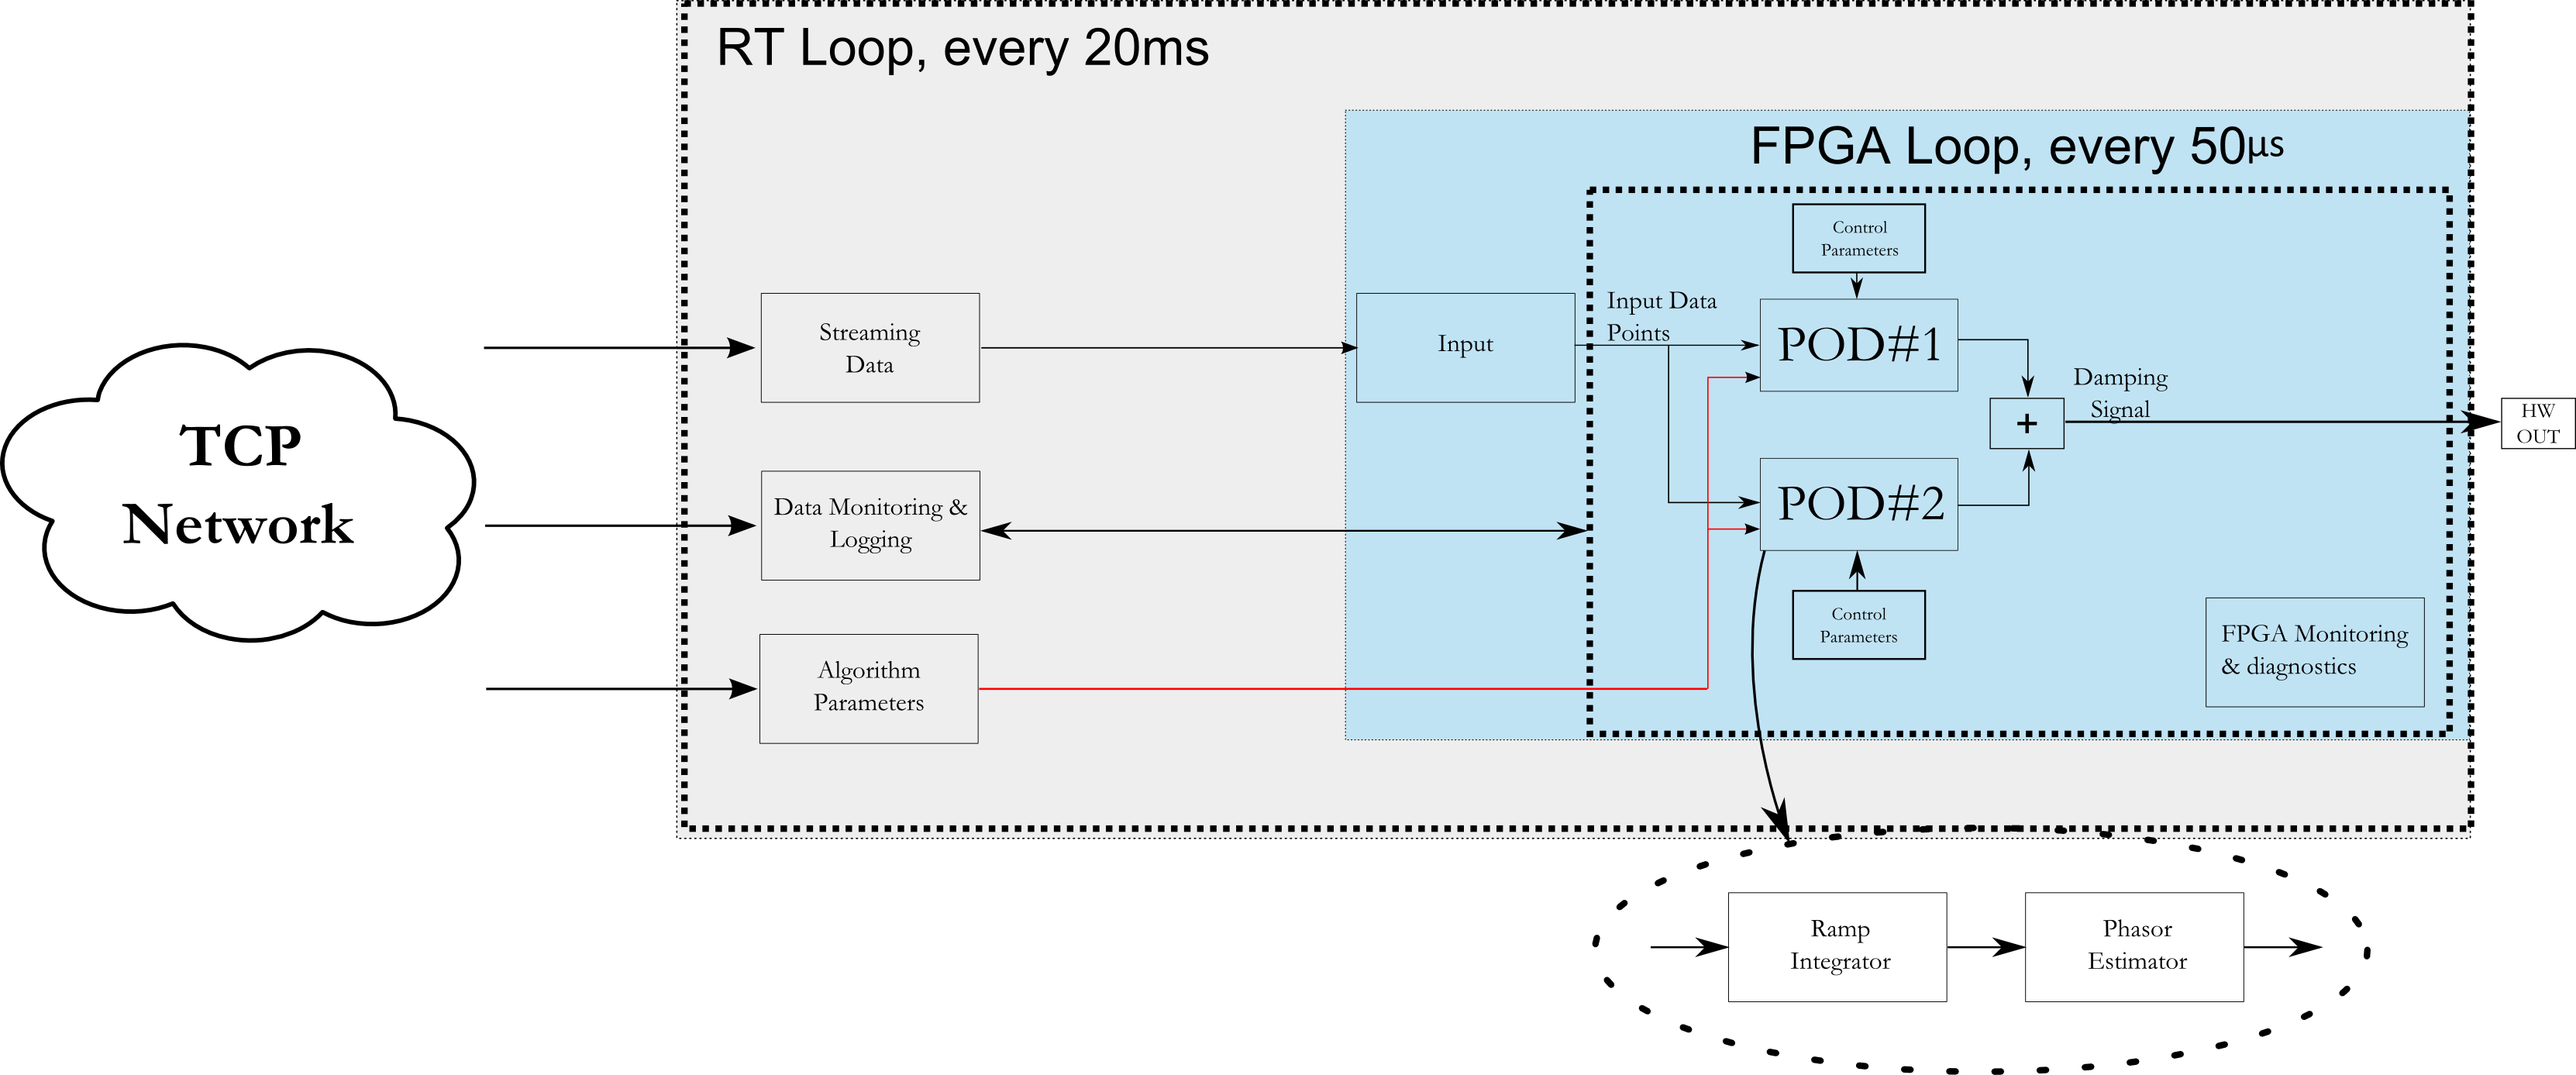
\includegraphics[width=3.5in]{FPGA_Block_Diagram.png} 
%\caption{Software Architecture of RT Controller}
%\label{RTSoftware}
%\end{figure}

The hardware implementation of the POD was based on the cRIO 9081 \cite{cRIO9081} from National Instruments. This controller is equipped with an on-board FPGA (maximum clock speed of 80Mhz\footnote{\url{http://www.xilinx.com/support/documentation/data_sheets/ds162.pdf}}) in addition to an independent real-time controller (1.06GHz Intel Celeron U3405). 
%update figure to show that Local control function was NOT implemented. Future work!-----------------------------------------------------------------------------
\begin{figure*}[thbp]
\centering
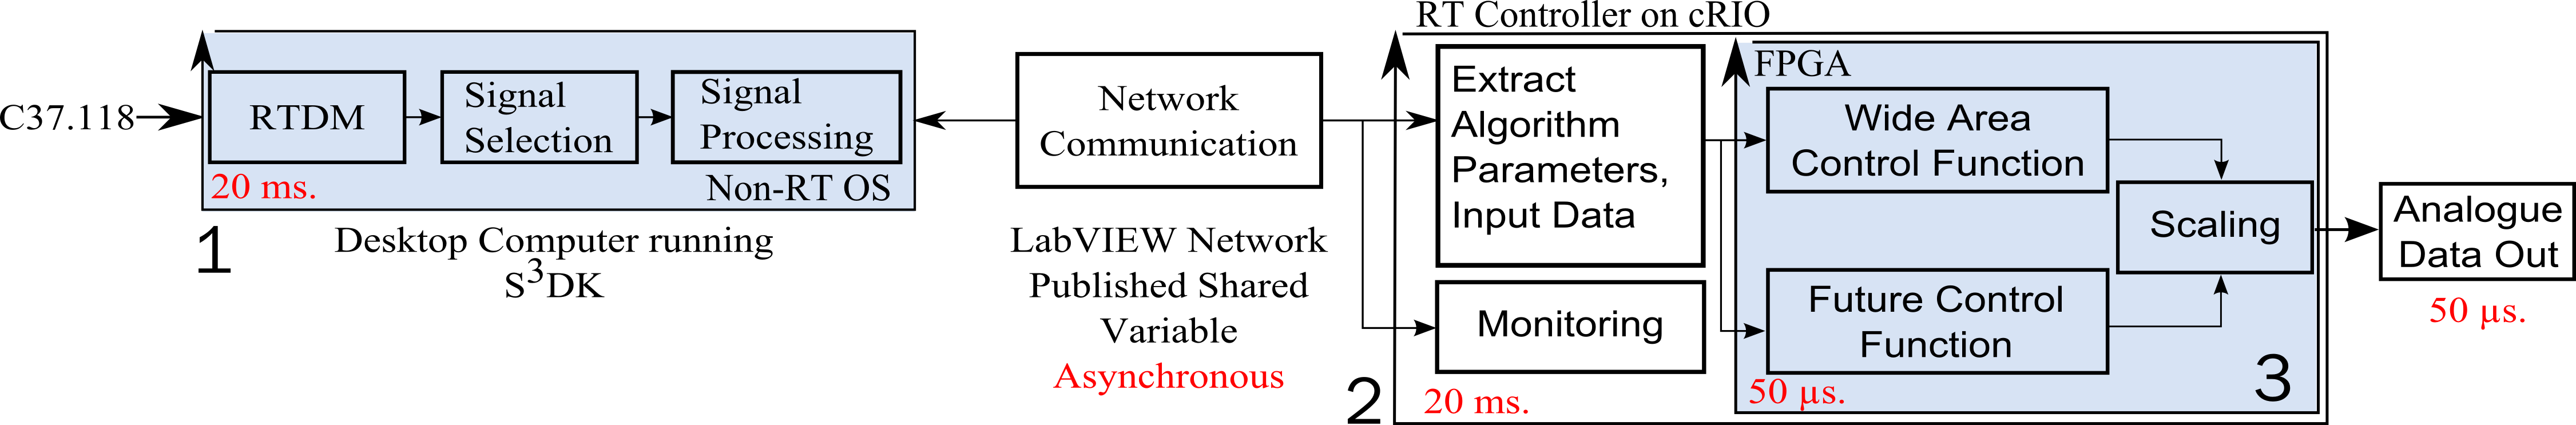
\includegraphics[width=5in]{Final_RT_Arch.png} 
\caption{Three-layer Software and Hardware Architecture of the WAPOD Controller. Loop rates are indicated in red.} %showing future expandability with Local control function
\label{RTArchitecture}
\vspace{-1em}
\end{figure*}

A three-layer, modular code architecture\cite{Rebello_WAPOD_Software}, following guidelines from the manufacturer \cite{LabviewTemplate}, was selected for implementation. An outline of the architecture is shown in Figure \ref{RTArchitecture} and each of the three layers are briefly described below (Corresponding to the numbers in Figure \ref{RTArchitecture}). 

\begin{enumerate}
\item Remote Interface: Runs on a standard, workstation computer. Used to input algorithm parameters and monitor data \& performance. Receives the aligned synchrophasor data stream and extracts measured value data. This  layer is non deterministic in time.

\item Real Time (RT) Software : Manages network communication to the remote interface and also generates performance monitoring data. The remote interface interacts with this layer over the communication network. Transfers extracted synchrophasor data to the FPGA.

\item Core FPGA Software : Interacts with hardware terminals for I/O and runs the Phasor-POD algorithm. Input data comes through the RT interface running on the cRIO.

\end{enumerate}

The Phasor-POD algorithm could be implemented on either the real-time section of the cRIO or the FPGA but was implemented on the FPGA. This decision was made keeping in mind the computational resources and response speed needed to match the step size of the real-time simulator. The complexity of the code meant that the cRIO\rq{s} real-time controller would not be able to complete each iteration of the algorithm in the required 50$\mu$s response time. The real-time section of the cRIO only handles network communication. Its primary purpose is to receive measurement data that the workstation computer extracts and to stream this data to the Phasor-POD algorithm running on the FPGA. The real-time controller also handles commands coming from the user interface running on the workstation computer.  It also monitors the output of the FPGA, sends data to the user interface for monitoring, periodically logs input and output data and handles error conditions.\\

The remote interface runs in LabVIEW on a conventional computer. The Phasor-POD algorithm can be controlled and monitored from this interface. The operating system here is not real-time but multi-tasking. The execution speed therefore depends on the processor load and is not deterministic. The  $S^{3}DK$ was used to unwrap the PMU streams coming from the PDC and extract phasor measurements. This allowed for data to be extracted and used directly in the LabVIEW environment. The PMU reporting rate was 50 messages a second and new data was available every 20ms. The loop rate used by the $S^{3}DK$ was therefore 20ms. The selection of an input signal for the controller and any signal processing required are performed here. For example, if active power is to be used as a POD input, voltage and current values must be multiplied to obtain the active power. If the voltage angle difference is to be used as an input, the required calculations are performed in this LabVIEW Virtual Instrument (VI\footnote{A LabVIEW program. See \url{http://www.ni.com/white-paper/7001/en/}}).
%Also, the algorithm parameters can be set and modified.
%This format for equations does not work. Why?---------------------------------

%\begin{equation} \label{phasoreqn}
%\left(t\right)={s}_{avg}+\mathrm{Re}\left\{{\stackrel{\to }{s}}_{ph}\cdot %{e}^{{j}^{wt}}\right\} \cite{Chaudhuri}
%\end{equation} 

%Include equation if needed---------------------------------

%$s\left(t\right)={s}_{avg}+\mathrm{Re}\left\{{\stackrel{\to }{s}}_{ph}\cdot {e}^{{j}^{wt}}\right\}$ \cite{Chaudhuri}

% An example of a floating figure using the graphicx package.
% Note that \label must occur AFTER (or within) \caption.
% For figures, \caption should occur after the \includegraphics.
% Note that IEEEtran v1.7 and later has special internal code that
% is designed to preserve the operation of \label within \caption
% even when the captionsoff option is in effect. However, because
% of issues like this, it may be the safest practice to put all your
% \label just after \caption rather than within \caption{}.
%
% Reminder: the "draftcls" or "draftclsnofoot", not "draft", class
% option should be used if it is desired that the figures are to be
% displayed while in draft mode.
%
%\begin{figure}[!t]
%\centering
%\includegraphics[width=2.5in]{myfigure}
% where an .eps filename suffix will be assumed under latex, 
% and a .pdf suffix will be assumed for pdflatex; or what has been declared
% via \DeclareGraphicsExtensions.
%\caption{Simulation Results}
%\label{fig_sim}
%\end{figure}

% Note that IEEE typically puts floats only at the top, even when this
% results in a large percentage of a column being occupied by floats.


% An example of a double column floating figure using two subfigures.
% (The subfig.sty package must be loaded for this to work.)
% The subfigure \label commands are set within each subfloat command, the
% \label for the overall figure must come after \caption.
% \hfil must be used as a separator to get equal spacing.
% The subfigure.sty package works much the same way, except \subfigure is
% used instead of \subfloat.
%
%\begin{figure*}[!t]
%\centerline{\subfloat[Case I]\includegraphics[width=2.5in]{subfigcase1}%
%\label{fig_first_case}}
%\hfil
%\subfloat[Case II]{\includegraphics[width=2.5in]{subfigcase2}%
%\label{fig_second_case}}}
%\caption{Simulation results}
%\label{fig_sim}
%\end{figure*}
%
% Note that often IEEE papers with subfigures do not employ subfigure
% captions (using the optional argument to \subfloat), but instead will
% reference/describe all of them (a), (b), etc., within the main caption.


% An example of a floating table. Note that, for IEEE style tables, the 
% \caption command should come BEFORE the table. Table text will default to
% \footnotesize as IEEE normally uses this smaller font for tables.
% The \label must come after \caption as always.
%
%\begin{table}[!t]
%% increase table row spacing, adjust to taste
%\renewcommand{\arraystretch}{1.3}
% if using array.sty, it might be a good idea to tweak the value of
% \extrarowheight as needed to properly center the text within the cells
%\caption{An Example of a Table}
%\label{table_example}
%\centering
%% Some packages, such as MDW tools, offer better commands for making tables
%% than the plain LaTeX2e tabular which is used here.
%\begin{tabular}{|c||c|}
%\hline
%One & Two\\
%\hline
%Three & Four\\
%\hline
%\end{tabular}
%\end{table}


% Note that IEEE does not put floats in the very first column - or typically
% anywhere on the first page for that matter. Also, in-text middle ("here")
% positioning is not used. Most IEEE journals use top floats exclusively.
% Note that, LaTeX2e, unlike IEEE journals, places footnotes above bottom
% floats. This can be corrected via the \fnbelowfloat command of the
% stfloats package.

\section{Experimental Setup Preparation}\label{SetupPreparation}

The nature of the Phasor-POD algorithm is generic enough to allow it to be used as a modulating input to a variety of controlled devices. Two examples are illustrated in this work, one, as a damping controller modulating a generator\rq{s} AVR system and the other as a modulating input to the excitation system of a FACTS device (here, an SVC). Figure \ref{NetworkOutline} illustrates both these uses along with the two-area network outline. Note that both functions are not implemented simultaneously.
\vspace{-0.5em}
\subsection{Two-Area Model Preparation - Generator AVR}

\begin{figure}[tbp]
\centering
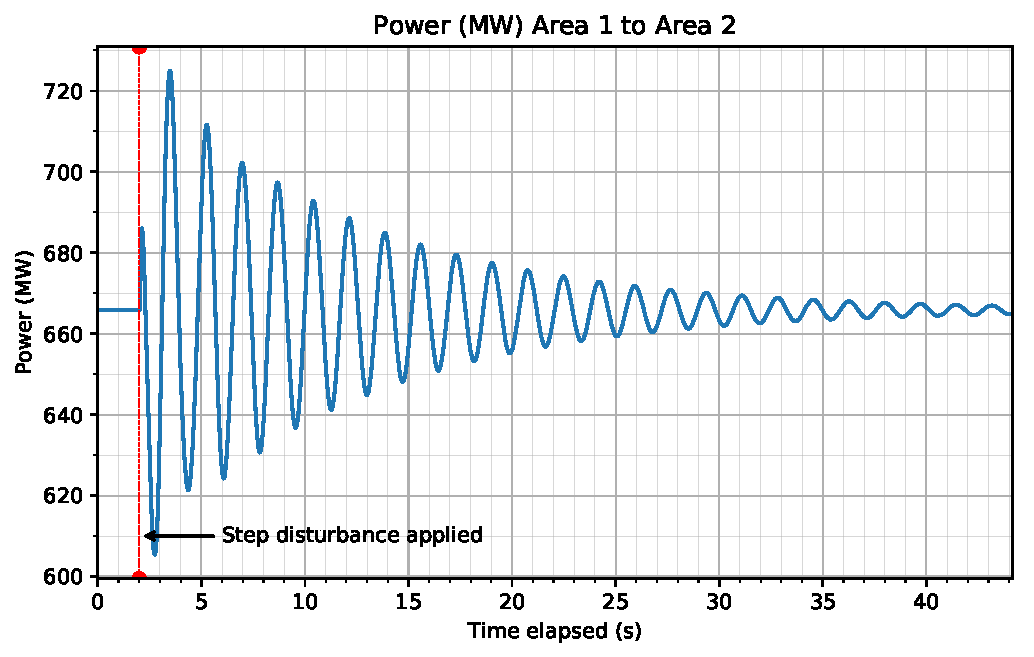
\includegraphics[width=3.5in]{PSS_degraded_response.pdf}
\caption{Damping performance of the base case PSS only at Machine M1. Local active power is used as the PSS input.}
\label{PSS_Degrade}
\vspace{-1em}
\end{figure}
%\vspace{-0.5em}

%The two-area network \cite{KundurTwoArea} is known to be unstable without external damping control. 
The original Klein-Rogers-Kundur model in \cite{KundurTwoArea} was modified for the studies in this work. In order to assess the performance of the WAPOD, the base case employs a damping control system (PSS) only at Machine M1 in Area-1 (see~Figure~\ref{NetworkOutline}). All other machines do not have a PSS installed. The WAPOD output is used as an additional input to machine M1\rq{s} AVR system. This configuration was  verified to be stable and is able to restore the system to stability after the application (and subsequent clearing) of an 8 cycle, three-phase to ground fault at bus 8 in Figure~\ref{NetworkOutline}. To demonstrate a potential application scenario for the developed POD prototype, the performance of the PSS was set up so that it is able to provide damping but with a long response and settling time (Figure \ref{PSS_Degrade}). This figure shows the system response to a 200 ms., 5\% perturbation in the voltage reference of machine M1. Note that under the action of the sole PSS at machine M1, the inter-area mode is damped and the system is restored to stability. This mimics a real-world situation with an already installed PSS whose performance has degraded over time due to changing network conditions or poor tuning. Using only one PSS ensures that the inter-area mode is clearly visible. Our intention with this modification is to demonstrate that a hardware implementation of the POD algorithm can improve system damping despite the controller\rq{s} real-world limitations. It is not our goal to demonstrate that a hardware-based controller is able to improve system damping with a PSS installed at each machine. Though this may be possible, this work only seeks to demonstrate that a hardware implementation of a Phasor-POD based on synchrophasor data is able to function as expected.

\begin{figure*}[!thpb]
\centering
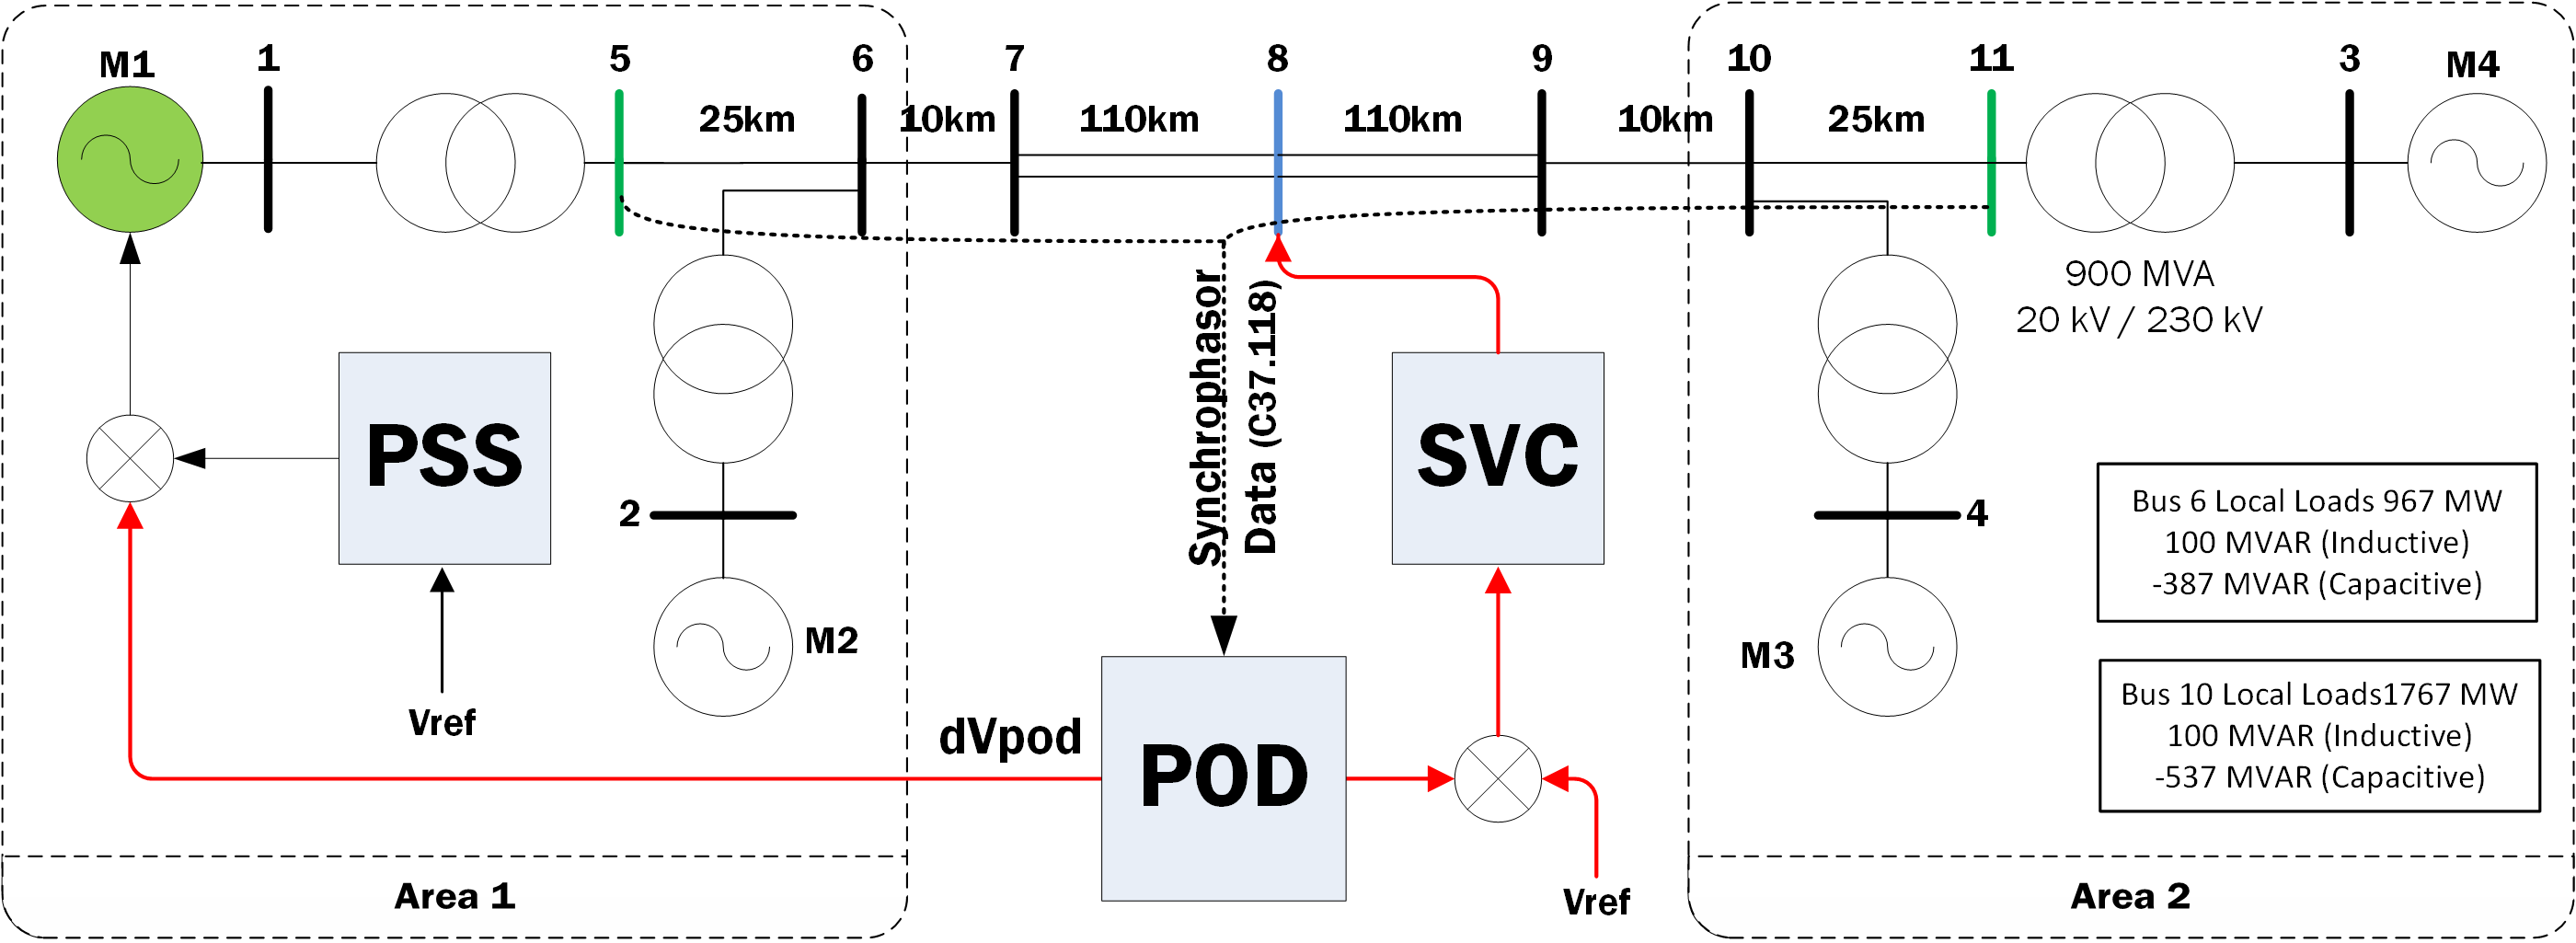
\includegraphics[width=5in]{Kundur2Area_outline_multi.png}
\caption{Modified Two-Area Four-Machine network outline showing PMU data sources and both uses of the POD damping output. Note that only one scenario is implemented at a time i.e. either generator or SVC modulation. Network details are left incomplete for illustration purposes.}
\label{NetworkOutline}
\end{figure*}

%The \textsc{Simulink} model used here implements damping control using a supplementary signal generated from a PSS and applied to the excitation system of each of the machines to achieve steady-state stability and also to damp out the inter-area mode.

%The difference between the rotational inertias of two of the machines, in an otherwise symmetric network gives rise to the 0.64Hz inter-area mode. 

%Details of the two-area model parameters are listed in Appendix \ref{LiiteC}.\\


\subsection{Two-Area Model Preparation - FACTS Device}

The second application in Figure \ref{NetworkOutline} is to use the WAPOD output as a modulating input to an SVC's excitation system. The two-area model was prepared for simulation in the same way as in the previous case, however, in this case a PSS was included at all four machines. The SVC model implemented was an average-value model, identical to that used in \cite{PhasorPODImplement}. The SVC was connected at the mid-point of the two area network (Bus 8 in Figure \ref{NetworkOutline}). As shown in \cite{sVARdamp}, this is the point where voltage swings will be the greatest and also where the SVC can be most effective at damping power flow swings. For comparison purposes, two parallel and identical implementations of the Phasor-POD algorithm were used, one implemented in \textsc{Simulink} and the other on the cRIO. Either could be switched in at a given time. It is important to note here that when the hardware-POD was switched in, the PSS's at each of the four machines were disconnected, leaving the SVC as the sole control and damping device in the network. The ability of the SVC to keep the network stable and also to restore it to stability was verified with off-line simulations using the Phasor-POD implemented in \textsc{Simulink}.% In addition, the performance of the PSS's were not modified as the Phasor-POD algorithm would not be running in parallel with them.

%\begin{figure}[!th]
%\centering
%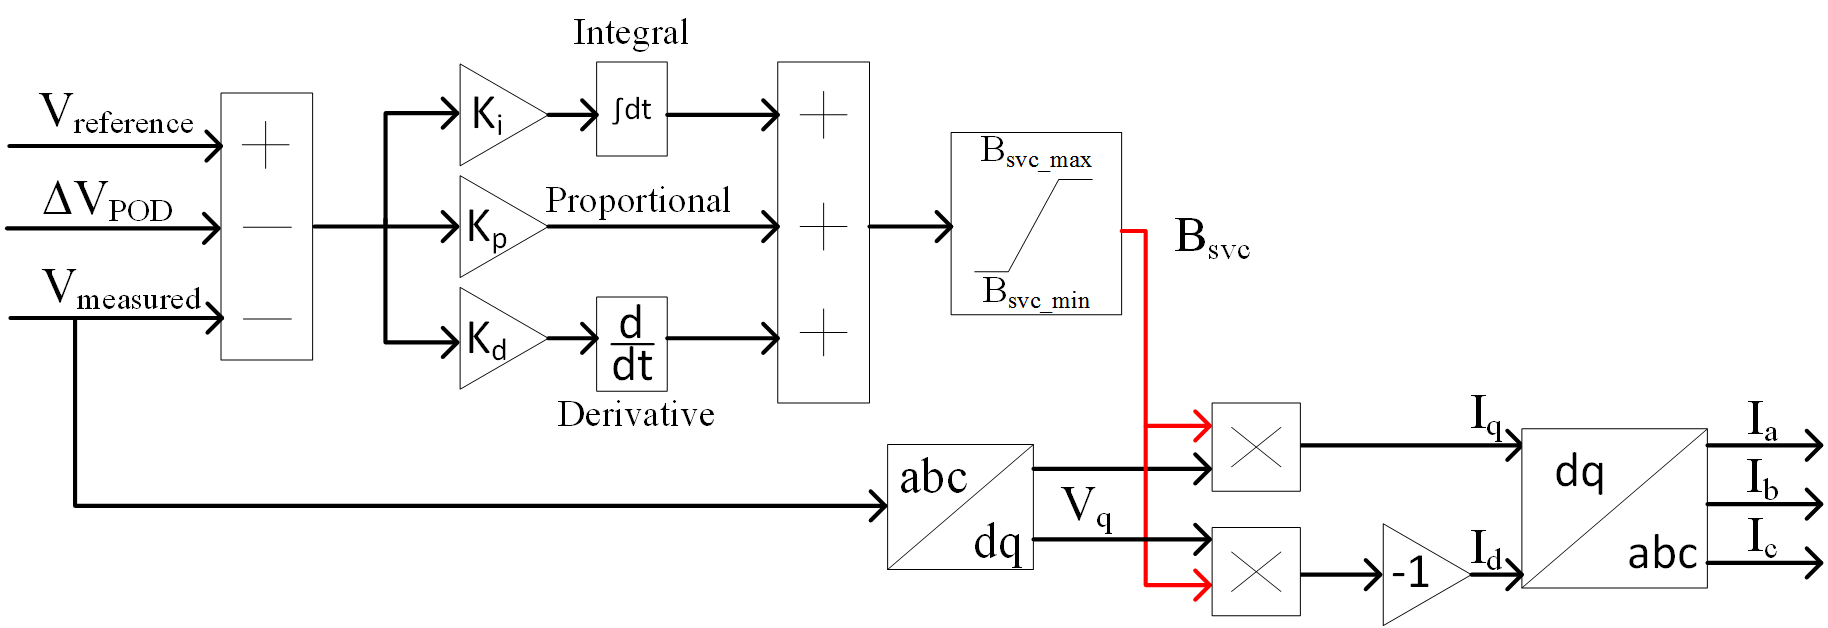
\includegraphics[width=3.5in]{SVC_AverageModel.png}
%\caption{Block Diagram for average-valued SVC model used}
%\label{SVC_Model}
%\end{figure}
\vspace{-0.7em}
\subsection{Real-Time Simulation}
The modified network in each case was grouped into sub-systems and prepared for simulation using RT-LAB \cite{eMEGASIM}. The simulation time step chosen was 50$\mu$s meaning that outputs and inputs of the real-time simulator were updated every 50$\mu$s. Current and voltage measurements were taken from the buses marked (in green) in Figure \ref{NetworkOutline} and were extracted via the analogue outputs of the real-time simulator. The damping signal \emph{dVpod} in Figure~\ref{NetworkOutline} was generated at two points; one in the real-time simulation itself using a \textsc{Simulink} implementation of the Phasor POD algorithm and one externally on the cRIO. Both signals were generated simultaneously and either one could be switched in for use in the simulation.

\section{Testing \& Results}\label{Results}
The POD algorithm implemented in \textsc{Simulink} uses locally available active power measurements as input. In the case of the Generator PSS, this is the active power measured at the terminals of the generator. In the case of the SVC, the active power at the mid-point of the interconnecting line (also the point of connection of the SVC) is used as an input. The WAPOD hardware prototype can use these same signals as inputs in each case but can also exploit other data from the synchrophasor data stream. Testing the operation of the hardware prototype involved using the HIL setup outlined in Figure~\ref{Hardware_Outline} and verifying whether steady-state stability could be maintained in the simulated two-area network. This test proved that the hardware prototype was able to prevent the existing inter-area oscillation mode from increasing in magnitude. Once this was demonstrated, the inter-area mode was excited by perturbing the voltage reference $V_{ref}$ of Machine M1. The oscillations caused by this disturbance would then be damped out by the proposed controller. Testing was carried out in several phases, one with the \textsc{Simulink} POD operational and the other with the cRIO-based WAPOD feeding in to the real-time simulation. In the latter case, three different damping inputs were tested: active power, positive sequence current magnitude and the voltage angle difference between buses 5 and 11 in Figure \ref{NetworkOutline}.
\vspace{-0.7em}
\subsection{SVC Excitation Supplementary Input}
Figure \ref{SVC_Plots} illustrates the response of the hardware controller to a small disturbance at machine M1. This disturbance is a 5\% change for 200 ms. in the reference voltage of the AVR. This is sufficient to excite the inter-area mode. The best damping performance is achieved using voltage angle difference as a damping input to the Phasor-POD algorithm. This supports the theoretical results discussed in \cite{Yuwa}. Response parameters such as settling times and overshoot were calculated based on the response in Figure \ref{SVC_Plots} and are presented in Table \ref{SVCResponseTable}. The response of the simulated POD (in \textsc{Simulink}) was used as a baseline to calculate the overshoot. The settling time is calculated as the time required for the response of the controller (in volts) to be constrained to +/- 1V.
%A frequency analysis of each of these responses shows that the dominant mode in each response is the 0.64Hz inter-area mode.\\
\begin{table}[!ht]
\caption{Response Parameters : SVC Excitation Supplementary Input}\label{SVCResponseTable}
\begin{center}
\begin{tabular}{|l|r|r|}
\hline \textbf{Input Parameter} & \textbf{Percentage Overshoot} & \textbf{Settling Time (s)} \\
\hline Simulated POD (Active Power)& N/A & 3.875 \\ 
\hline Active Power & 290.05 & 13.94 \\ 
\hline Pos. Seq. Current & 142.67 & 16.95\\ 
\hline Voltage Angle Diff. & -11.26 & 9.66\\ 
%\hline POD - FPGA & 50$\mu$s & Real Time \\ 
\hline 
\end{tabular}
\end{center}
\vspace{-1em}
\end{table}  

%This is evident in Figure \ref{FourierAngle}, which presents the magnitude spectrum of the controller response with voltage angle as input.

\begin{figure}[thpb]
\centering
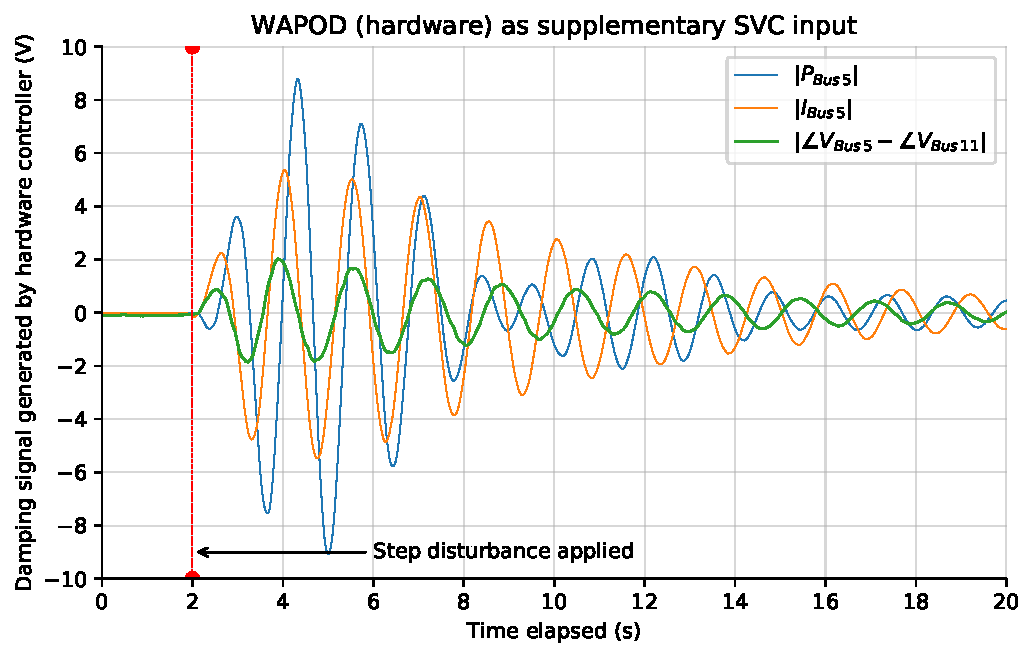
\includegraphics[width=3.5in]{Controller_Response_SVC_input.pdf}
\caption{Controller Response Comparison : Supplementary SVC Excitation Input}
\label{SVC_Plots}
\vspace{-1em}
\end{figure}
%\vspace{-0.5em}
%\begin{figure}[!th]
%\centering
%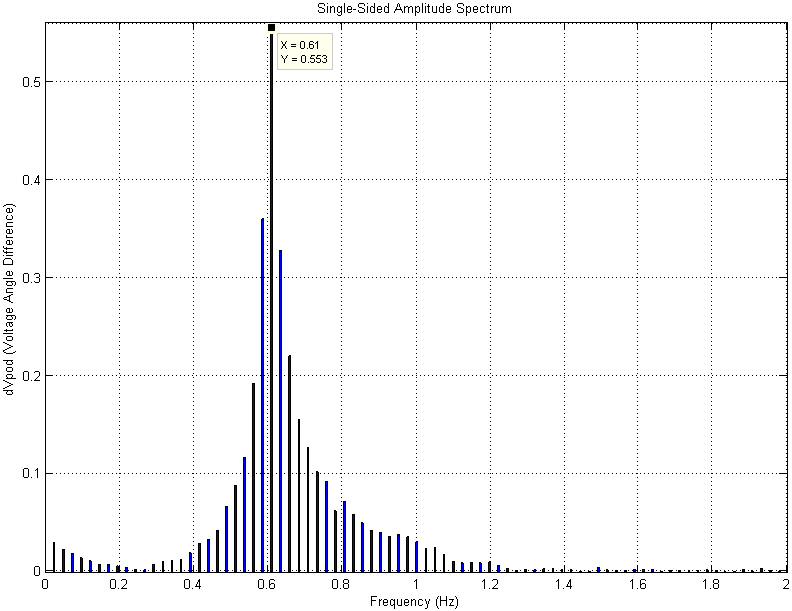
\includegraphics[width=3.5in]{VoltageAngleDiff.png}
%\caption{Controller Response Comparison : Supplementary SVC Excitation Input}
%\label{FourierAngle}
%\end{figure}

All data presented in Figure \ref{SVC_Plots} was captured in the real-time simulator. Data was also recorded at other locations in the simulation such as at the PDC but these have a lower time resolution and are thus not presented here. As further proof of the results presented in this work, the output of the hardware controller is captured directly using an oscilloscope (Figure \ref{ScopeCapture}).

\begin{figure}[thbp]
\centering
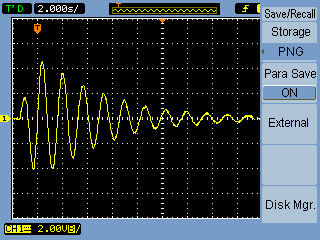
\includegraphics[width=2.5in]{Best_sample.png}
\caption{Controller Response with Voltage Angle Difference input Captured using an Oscilloscope}
\label{ScopeCapture}
\vspace{-1em}
\end{figure}

\subsection{Generator Excitation Supplementary Input}
The controller response to a small disturbance when operating in tandem with a degraded PSS is shown in Figure~\ref{Generator_Plots}. It can also be noted that the response of the damping signal is significantly different from that in Figure~\ref{SVC_Plots}, where the dominant 0.64Hz mode is clearly visible. Also evident from Figure~\ref{Generator_Plots} is the fact that the damping performance of the WAPOD changes significantly as its input is changed. Using the voltage angle difference as input provides the best performance. The performance of the WAPOD with the voltage angle difference input is very close to the performance of the simulated POD algorithm that uses local active power as input. This performance is achieved despite the presence of a stochastic time delay and noise in the input measurements of the WAPOD. As in the case with the SVC, the theoretical results in \cite{Yuwa} agree with the experimental results presented here.

\begin{figure}[thpb]
\centering
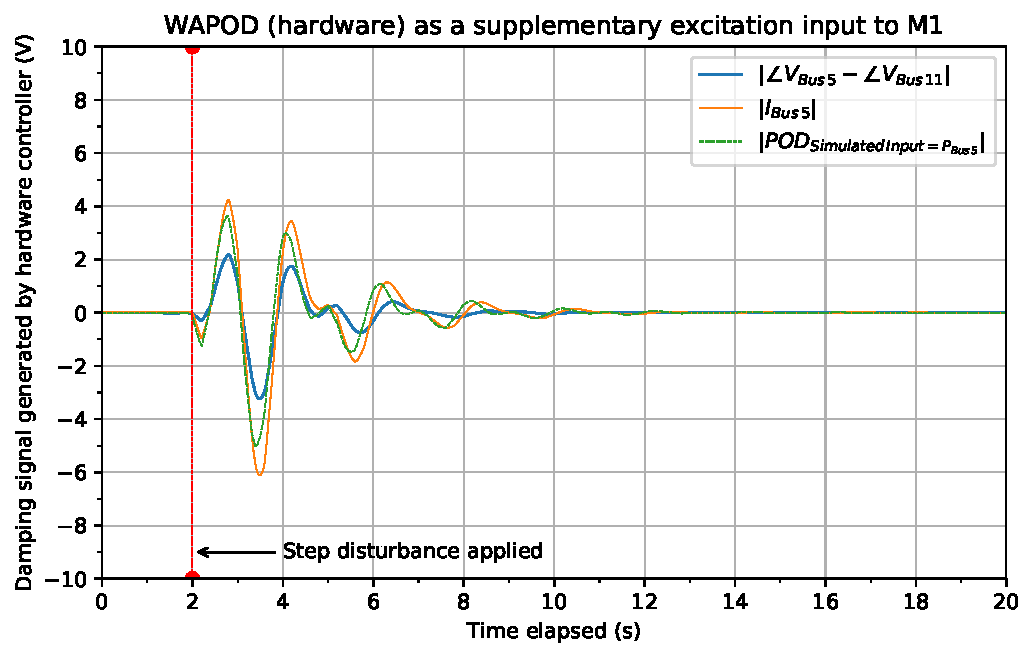
\includegraphics[width=3.5in]{Controller_Response_Generator_input.pdf}
\caption{Controller Response Comparison : Supplementary Generator Excitation Input}
\label{Generator_Plots}
\vspace{-1em}
\end{figure}
%\vspace{-1em}

As in the previous case, response parameters such as settling times and overshoot were calculated based on the response in Figure \ref{Generator_Plots} and are presented in Table \ref{GENResponseTable}. Definitions are identical to the previous case.\\

\begin{table}[!ht]
\caption{Response Parameters : Supplementary Generator Excitation Input}\label{GENResponseTable}
\begin{center}
\begin{tabular}{|l|r|r|}
%\hline \textbf{Element} & \textbf{Loop Rate} & \textbf{Mode} \\
\hline \textbf{Input Parameter} & \textbf{Percentage Overshoot} & \textbf{Settling Time (s)} \\
\hline Simulated POD (Active Power) & N/A & 6.26\\ 
\hline Active Power & 0.10 & 6.41\\ 
\hline Pos. Sequence Current & 23.46 & 6.53 \\ 
\hline Voltage Angle Diff & -34.72 & 5.20 \\ 
%\hline POD - FPGA & 50$\mu$s & Real Time \\ 
\hline 
\end{tabular}
\end{center}
\end{table}  
\vspace{-2em}
%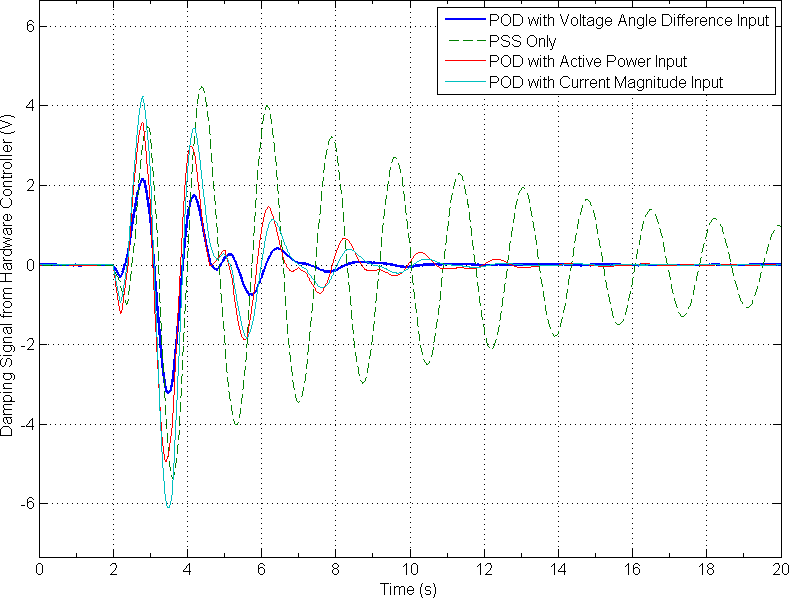
\includegraphics{Wide_Area_ResponseComparison_SamePlot.png} 

%\section{Additional Inputs}
%\pbox{20cm}{This is the first \\ cell}
%\vtop{\hbox{\strut top line}\hbox{\strut botline}}

\section{Challenges of a real-world implementation}\label{Challenges}

\subsection{Time Delays}

The Phasor POD algorithm implemented in \textsc{Simulink} has close to zero time delay between the power system changing and the controller responding. The same algorithm, when run on the cRIO, receives input data with a stochastic delay. It is evident from Figure~\ref{Hardware_Outline} that several sources of stochastic time delay exist. Sections such as the analogue amplifiers, the FPGA (50$\mu$s) and the real-time section of the cRIO all represent fixed, non-zero time delays. Elements such as the D/A and A/D conversion in the real-time simulator also add a deterministic time delay. However, elements in the data path such as TCP/IP network communication and the PC used to extract raw measurement data from the PDC synchrophasor stream all represent variable delays. The total delay allows for a network disturbance to grow slightly before the controller begins to respond. This delay also changes the phase compensation required in the Phasor-POD algorithm. The phase compensation needed can be changed from the remote interface, depending on the measured delay. The experimentally measured end-to-end delay over the complete data path in Figure \ref{Hardware_Outline} averaged 344 ms. This was calculated by logging data in the real-time simulator and measuring the delay between the power system response and the controller response (Fig. \ref{varying_time_delay}). Presently, the phase compensation required is determined iteratively and off-line, however, this can be automated using time-stamped data together with an adaptive controller.

\begin{figure}[thpb]
\centering
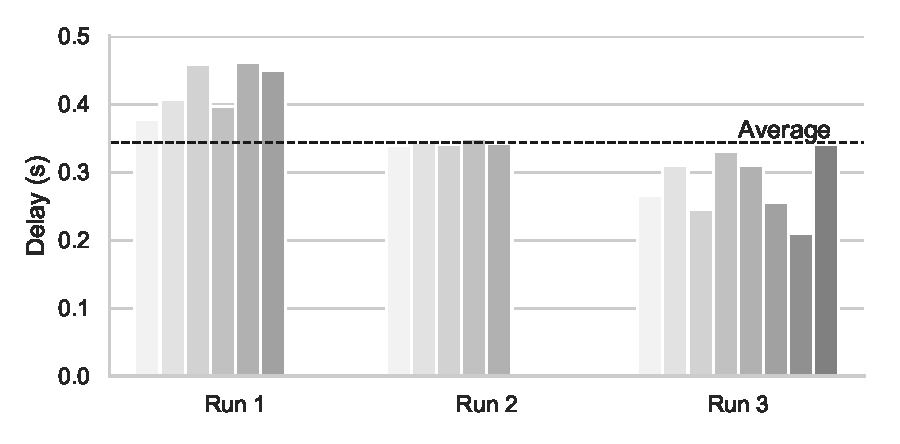
\includegraphics[width=3in]{delay_bar_chart.pdf}
\caption{Time delay measurements for 19 HIL experiments}
\label{varying_time_delay}
\vspace{-1em}
\end{figure}

%\begin{table}[h]
%\caption{Signal Propagation Delay Calculation}\label{DelayData}
%\begin{center}
% \begin{tabular}{|c|r|r|c|}
%  \hline \multicolumn{1}{|p{1cm}|}{\centering \textbf{Pulse \\ Number}} & \multicolumn{1}{|p{2cm}|}{\centering \textbf{Simulated POD \\ Response Start\\} (s)} & \multicolumn{1}{|p{2cm}|}{\centering \textbf{cRIO POD \\ Response Start} \\(s)} & \multicolumn{1}{|p{2cm}|}{\centering \textbf{Time Delay} \\ (ms) } \\ 
% \hline 1 & 60.01 & 60.28 & 265 \\ 
% \hline 2 & 70.04 & 70.35 & 310 \\ 
% \hline 3 & 80.02 & 80.27 & 245 \\ 
% \hline 4 & 90.04 & 90.37 & 330 \\ 
% \hline 5 & 100.04 & 100.35 & 310 \\ 
% \hline 6 & 110.03 & 110.29 & 255 \\ 
% \hline 7 & 120.05 & 120.26 & \textbf{210} \\ 
% \hline 8 & 130.02 & 130.36 & \textbf{340} \\ 
% \hline 
% \end{tabular}\label{ex:DelayData}
%\end{center}
%\vspace{-1.5em}
%\end{table} 

%\vspace{-2em}

%In a direct comparison between the simulated Phasor-POD and one running on the cRIO, the time delay will be 

\subsection{Analogue Limits and Noise}
The original POD algorithm~\cite{PhasorPOD} was developed and simulated in an ideal, noise-free environment with zero delay (\textsc{Simulink}). More importantly, no limits are imposed on the magnitude of either the controller's inputs or outputs. In contrast, a hardware-based implementation as in this paper, usies analogue signals and thus is constrained by analogue signal limits (see Figure \ref{ScalingProblem}). Consider the analogue outputs of OPAL-RT's eMEGASIM simulator which are rated for $\pm16V$ or $\pm10mA$  \cite{eMEGASIM}. In contrast, the standard input modules of typical PMU's are rated for 0-300V. A 0-16V analogue signal will not occupy a significant dynamic range of the PMU\rq{}s inputs. Additionally, a signal of such a small magnitude will be contaminated by noise and will consequently have a poor Signal-to-Noise ratio. A similar argument can be made for the analogue current outputs. Our solution involved amplifying the analogue signals from the real-time simulator to levels that used more of the dynamic range of the PMU input modules. This simultaneously improves both accuracy and the signal-to-noise ratio.

\begin{figure}[tphb]
\centering
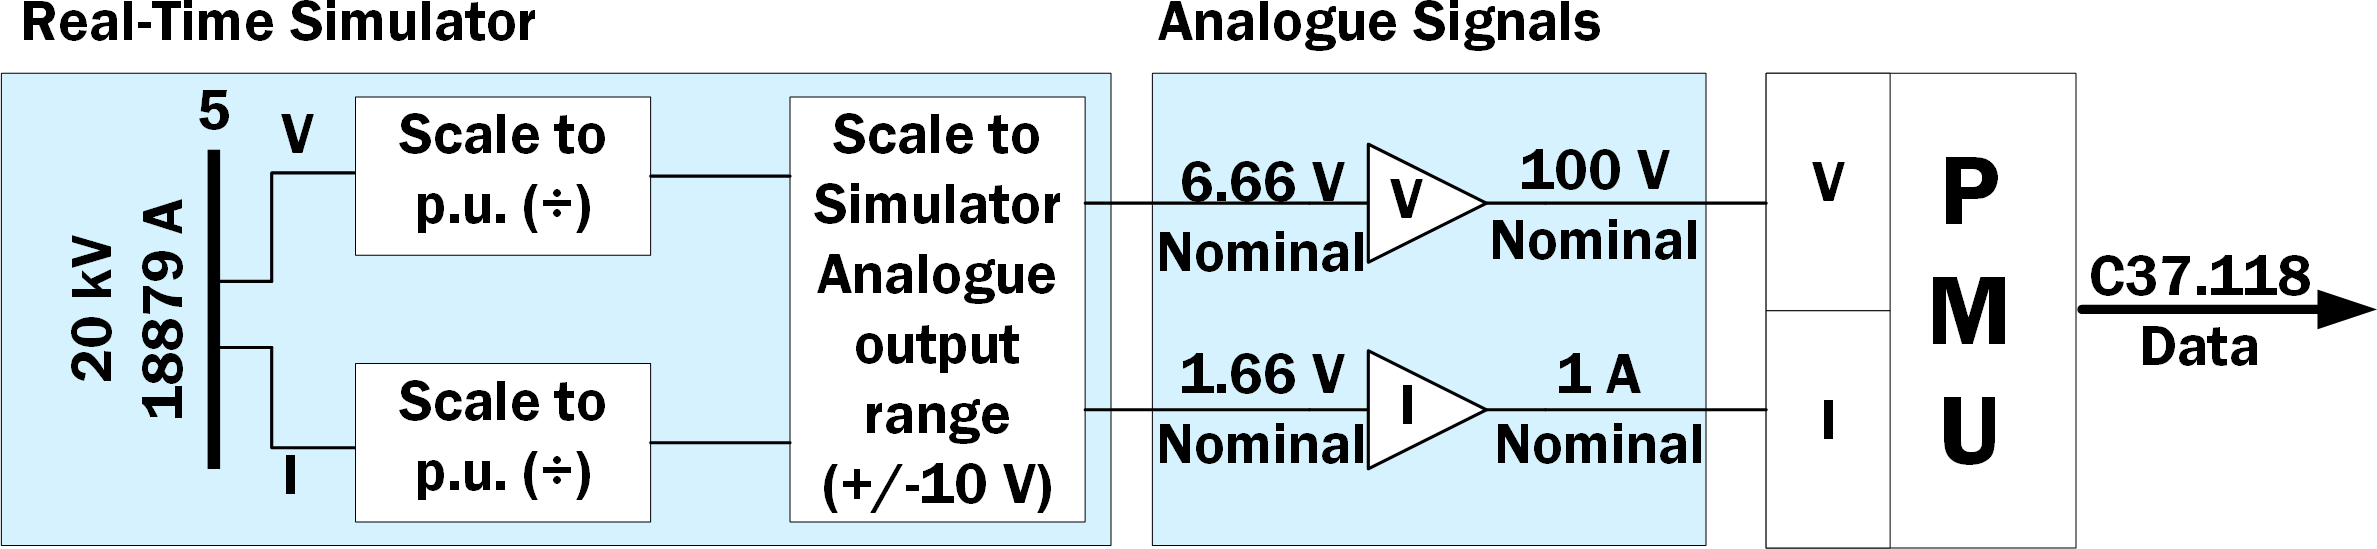
\includegraphics[width=3.5in]{Scaling.png}
\vspace{-1.3em}
\caption{Signal Scaling at each step of simulation}
\label{ScalingProblem}
\end{figure}
\vspace{-0.4em}
The output of the simulated POD can vary over several orders of magnitude, ranging from $10^{5}$ p.u.. at times of peak damping to as small as $10^{-3}$ p.u. once the oscillation magnitude  becomes small. It is difficult to accurately recreate this output as an analogue signal with such a vast dynamic range. The voltage output module used here had a 24-bit resolution and was limited to $\pm 10V$ in magnitude. Any values generated by the POD algorithm that were greater in magnitude that 10V would cause output saturation. All these issues meant that signal magnitudes had to be amplified in certain cases to use the full measurement ranges or had to be limited in other cases, so as to capture variations without saturation. This was because a hard-wired POD output was used in our experiment. A solution would be to transmit the POD output digitally.

\subsection{Loop Rates and FPGA Resources}\label{looprate}
The most significant challenge in the real-time implementation of the Phasor-POD algorithm was the fact that different sections of the hardware loop ran at different loop rates or step sizes (see Figure \ref{RTArchitecture}). Added to this was the fact that the real-time simulator generated data every 50 $\mu$s (and thus expected data from the HIL set-up at the same rate) while the rest of the HIL set-up did not support such a high data rate. The PMUs used supported a maximum reporting rate of 50 samples/second. Table~\ref{ex:LoopRates} lists the different components of the HIL set-up together with their respective loop rates.
\begin{table}[htpb]
\caption{Comparison of Loop Rates of Different Components}\label{ex:LoopRates}
\begin{center}
\begin{tabular}{|l|r|c|}
\hline \textbf{Element} & \textbf{Loop Rate} & \textbf{Mode} \\
\hline OPAL-RT Simulator & 50$\mu$s & Real Time \\ 
\hline PMU (cRIO) & 20ms & Real Time \\ 
\hline Workstation Computer& 20ms & Not Real Time \\ 
\hline PDC & 20ms & Not Real-Time \\ %check data here
\hline POD - RT Section & 20ms & Real Time \\ 
\hline POD - FPGA & 50$\mu$s & Real Time \\ 
\hline 
\end{tabular}
\end{center}
\vspace{-1em}
\end{table} 


50 $\mu$s. was chosen for the FPGA loop rate to match the loop rate of the real-time simulator. This ensures that data was always available at the analogue input of the real-time simulator and that no erroneous data points were read. The 50 $\mu$s. loop rate of the FPGA meant that new input data was expected every 50 $\mu$s., corresponding to a 20000 samples/s PMU sampling rate. The first limitation was the execution speed of the real-time section of the cRIO, which was limited to 1ms, significantly slower than the FPGA\rq{s} speed. Further, new synchrophasor data was available from the PMUs only every 20 ms. One solution to this problem was up-sampling synchrophasor data. The major drawback of this method was that the up-sampling process on the RT controller is computationally intensive and would not run at the required 20 ms. loop rate. An alternative solution was a sample-and-hold algorithm implemented on the FPGA. The FPGA simply holds any data received by it till new data arrives. This was implemented and found to work satisfactorily. %The difference between the Phasor-POD algorithm running the \textsc{Simulink} simulation and that on the cRIO was the data rates of their respective input data. The simulated POD received new data every 50 $\mu$s. while the cRIO-based POD received data every 20 ms.

\subsection{FPGA Numeric Data Formats and Accuracy}

While the FPGA is a fast, deterministic and reliable computational device, it brings with it some limitations. Most of these arise from the fact that an FPGA has no operating system and all circuit logic is directly implemented in hardware. All computations are performed at the bit level, limiting the amount and complexity of computations that can be performed. Functions such as division or multiplication consume significant space on the FPGA\cite{LabViewManuals}. The FPGA on the cRIO9081 implements a numeric representation called Fixed Point\cite{LabViewManuals}. Here, the number of bits assigned to represent the integer and fractional part of a number is fixed before code execution\cite{LabViewManuals}. This assignment must be done in advance of code execution and the FPGA as a whole uses one fixed-point accuracy.

%This representation is similar to binary in the sense that increasing and decreasing powers of 2 are used to represent the integer and fractional parts of a number, respectively.

Fixing the number of bits used for fractions in the fixed-point representation is constrained by several factors such as the FPGA\rq{s} analogue outputs, which have finite limits. This limits the maximum integer part of the numbers used in the fixed point representation. Problems arise, however, when handling input to the POD algorithm as its magnitude it not constrained by analogue limits. Observe from Figures\ref{Hardware_Outline} and \ref{RTArchitecture} that input data to the POD algorithm is digital and is transmitted over a TCP/IP network. This is the challenge with determining the fixed point representation used on the FPGA. Using too many bits for the integer part of the number results in poor fractional accuracy which is important as the analogue outputs have finite limits. Using too few bits for the integer part of the number results in possible rounding and overflow conditions when working with large input data values.

%Floating point calculations, although possible, consume significant space on the FPGA and are typically slower than corresponding fixed-point calculations\cite{LabViewManuals}. Trigonometric functions such as a sine or cosine can be implemented using specifically designed code that takes several clock cycles to execute. A trade-off has to be made between code execution speed and accuracy. The Phasor POD algorithm implemented in this work uses floating point calculations, multiplication, division operations and  trigonometric operations.

%Due to the FPGA design, not all these calculations can be performed in the same data format. The FPGA-specific data format, the Fixed Point representation, is used to optimise complex computations such as those required in trigonometric functions. The drawback of this representation is that a trade-off must be made between the accuracy achieved and the range of values that can be represented. Keeping in mind the fact that the input values to the POD algorithm are not necessarily limited in magnitude, the POD algorithm is implemented using Floating-point numbers. Certain functions used in the algorithm, such as trigonometric functions, use FPGA-optimised code and require input and output in the fixed-point representation. Conversion between these two formats (Fixed and Floating point) sometimes results in rounding errors. The floating-point format includes a representation for calculations that result in infinite or complex values, called \texttt{NaN} (Not a Number)\cite{LabViewManuals}. This representation is not available in the fixed-point format and conversion results in errors.
%The most common result is that a conversion from a floating-point NaN results in a fixed-point number where all the bits are \texttt{1}. This produces a finite number and is incorrect. 

%A significant problem here was the fact that the synchrophasor data-extraction software running the on the workstation computer was not running in real-time. This, together with the TCP/IP sections, introduced stochastic delay in the control loop. 
%----------------------------------------------------------------------------------------------------------------------------------------------
\section{Further Work}\label{Future}

%The WAPOD prototype as developed in this work together with the experimental tests provides emperical evidence of the possibilities and benefits of using wide area synchrophasor data for damping control, as theorised in \cite{Yuwa}. 
This prototype is dependent on manual signal selection and algorithm parameter value calculation. These two processes can be automated by having the WAPOD itself monitor the various input signals and intelligently select the one having the highest observability of a particular mode \cite{Yuwa}. The algorithm parameters, including the required phase compensation can also be determined adaptively on the WAPOD itself. On the same lines, this can further be extended to include selection among available measurement locations on the network. The fact that a stochastic time delay is introduced by unwrapping the synchrophasor data stream on a desktop computer can be addressed by performing this function on the WAPOD controller (here, the cRIO) itself thus making the whole control loop more deterministic which is part of on-going work \cite{Audur}. 

\section{Conclusion}\label{Conclusion}
This work has provided experimental results showing the feasibility and benefits of using wide-area power system measurements as an input to an oscillation damping controller. The generic nature of the developed controller was demonstrated by using an identical implementation with mere changes in parameters to suit the controlled device's input requirements and capabilities. The hardware prototype developed on the NI cRIO was tested in a real-time HIL setup and was demonstrated to work satisfactorily. Real-world constraints such as time delays and signal conditioning were replicated as closely as possible. The flexibility of synchrophasor data was demonstrated and the wide range of inputs possible from this were also tested. The results from this work serve as experimental proof-of-concept to the theory presented in \cite{Yuwa} and pave the way for the development of other PMU-based real-time control systems.

% if have a single appendix:
%\appendix[Proof of the Zonklar Equations]
% or
%\appendix  % for no appendix heading
% do not use \section anymore after \appendix, only \section*
% is possibly needed

% use appendices with more than one appendix
% then use \section to start each appendix
% you must declare a \section before using any
% \subsection or using \label (\appendices by itself
% starts a section numbered zero.)
%


\appendices
%\section{Proof of the First Zonklar Equation}
%\section{Two Area Four-Machine Model Parameters\label{LiiteC}}
%
%Two-area model parameters (Similar to those used in \cite{KundurTwoArea})\\
%%\renewcommand{\theequation}{C\arabic{equation}}
%%\setcounter{equation}{0}  
%%\renewcommand{\thefigure}{C\arabic{figure}}
%%\setcounter{figure}{0}
%%\renewcommand{\thetable}{C\arabic{table}}
%%\setcounter{table}{0}
%
%\begin{table}[!ht]
%\caption{Common Generator Parameters used in Simulink Two Area Model}
%\begin{center}
%%\bigskip
%\begin{tabular}{|c|c|c|c|c|c|}
%
%\hline $ X_{d} $ & 1.8  &$ {X}_{d}^{\prime } $  & 1.8  & $ {X}_{d}^{\prime \prime } $ & 0.25  \\ 
%\hline $ X_{q} $ & 1.7  &$ {X}_{q}^{\prime } $  & 0.55 & $ {X}_{q}^{\prime \prime } $ & 0.25 \\ 
%\hline $ X_{l} $ & 0.2  & $ R_{a} $ & 0.0025  & $ K_{d} $  & 0 \\ 
%\hline $ {T}_{d0}^{\prime } $ &8s  & $ {T}_{q0}^{\prime } $ & 0.4s & - & - \\ 
%\hline $ {T}_{d}^{\prime \prime } $ & 0.03s & $ {T}_{q}^{\prime \prime } $ & 0.05s  &- &-  \\ 
%\hline $ A_{SAT} $& 0.015 & $ B_{SAT} $ & 9.6 & $ \psi_{T1} $  & 0.9 \\ 
%\hline 
%\end{tabular}
%\end{center}
%\end{table}
%\emph{N.B. All Parameters in p.u., on Generator Base}\\
%
%Step Up Transformer Impedance : $0+j0.15$\\
%
%\begin{table}[!ht]
%\caption{Transmission line parameters}
%\begin{center}
%\begin{tabular}{|c|c|}
%\hline $r=0.0001$ pu/km & $x_{l}=0.001$ pu/km \\
%\hline $b_{c}=0.00175$ pu/km &  Nominal Voltage : 230kV\\ 
%\hline 
%\end{tabular}
%\end{center}
%\end{table}
%
%\begin{table}[!ht]
%\caption{Self-excited DC exciter Parameters (common to all generators)}
%\begin{center}
%\begin{tabular}{|c|c|c|c|}
%\hline  $ K_{A} = 20 $& $ T_{A} = 0.055 $ & $ T_{E} = 0.36 $ & $ K_{F} = 0.125 $ \\ 
%\hline $ T_{F} = 1.8 $ & $ A_{ex} = 0.0053 $ & $ B_{ex} = 1.075 $ & $ T_{R} = 0.05 $ \\ 
%\hline 
%\end{tabular} 
%\end{center}
%\end{table}
%% you can choose not to have a title for an appendix
%% if you want by leaving the argument blank
%\section{Modifications Made to PSS Model}
%
%The default simulation model supplied with the \texttt{power\_PSS} example in \textsc{Matlab} has three types of PSS models \cite{MATLABexample} : an MB-PSS, a $\Delta\omega $-PSS and a $\Delta P_{a}$ PSS. The comparison of the three as presented in \cite{MATLABexample} concludes that the performance of the MB-PSS is the best. This model is thus, not used when modulating the PSS output with the Phasor-POD algorithm. Instead, the $\delta P_{a}$ PSS is used. The PSS model here is the generic PSS model available with SimPowerSystems \cite{PSSDocumentation}.\\
%
%The input to the $\Delta\omega $-PSS is the rotor speed deviation $\Delta\omega $. For an accurate comparison, this was changed to the measured active power measured at the generator terminals, $P_{a}$. The lead-lag block parameters were also changed from $\frac{1 + 50x10^{-3}s}{1 + 1s}$ to $\frac{1 + 50x10^{-3}s}{1 + 6s}$. Parameters here were determined iteratively. The change to the lead-lag block produces the effect in Figure \ref{PSS_Degrade} where the PSS is still able to restore the system to stability but takes almost a minute to damp out the oscillations versus approximately three seconds in the ideal case.\\

%Photos should span two columns or full page.

%\section{SmarTS Lab Outline}

%The SmarTS Lab at KTH was set up with the aim of developing wide area monitoring, protection and control (WAMPAC) schemes for the power grid. Much of the infrastructure and activities involve PMU data and the associated communication and computer systems  \cite{SmarTSLab}. The lab is equipped with facilities for real-time (RT) simulations and also RT Hardware-in-the-loop (HIL) tests. A reduced schematic is shown in Figure \ref{fig:SmarTSlabOutline}

%The core of the setup is the eMEGASIM Real-time simulator from OPAL RT ~\cite{eMEGASIM}. Two \textquoteleft targets' are available,  each running a 12-core 3.3Ghz Intel i7 processor \cite{SmarTSLab}. This allows the running of models created in \textsc{Matlab}/Simulink in real-time. These simulations can interact with external devices through the simulator's low-power analogue outputs and inputs or with data streamed over TCP/IP, UDP etc \cite{SmarTSLab}. In this thesis, the power system under test is simulated on this platform.\\

%The analogue outputs and their ratings are listed below:\label{OPALlimits}
%
%\begin{itemize}
%\item \textbf{Analogue Outputs} : 32 (+/-16V and +/-10mA)
%\item \textbf{Analogue Inputs} : 128 (+/-100V and +/-10mA)
%\end{itemize}

%The full listing of the SmarTS Lab, the simulator's capabilities and its interfaces is covered in \cite{PhasorPODImplement} and \cite{SmarTSLab}. The reader is referred to these sources for a more detailed of the hardware described here.
%The WAMPAC platform includes a Phasor Data Concentrator (PDC) and its associated software from Schweitzer Engineering Laboratories (SEL). Other devices are interfaced with the PDC such as protection relays with embedded PMU functionality, line differential protection relays (ABB), Compact RIO micro-controllers (National Instruments) and analogue signal amplifiers (Megger)\cite{SmarTSLab}. The hardware list here is incomplete and other devices are also used such as a GPS receiver, a relay current and voltage injection kit etc.

%\begin{figure*}[!t]
%\label{SetupImage}
%\centering
%\includegraphics[width=1\linewidth]{./LabView_Numbered}
%\caption{Outline of the SmarTS Lab. Corresponding to Numbers: 1: Real Time Simulator, 2: PDC Interface, 3: cRIO Tray, 4: Oscilloscope, 5: Analogue Signal Amplifiers, 6: SEL Protection Relays}
%\label{fig:LabView_Numbered}
%\end{figure*}

%\begin{figure*}[!t]
%\centering
%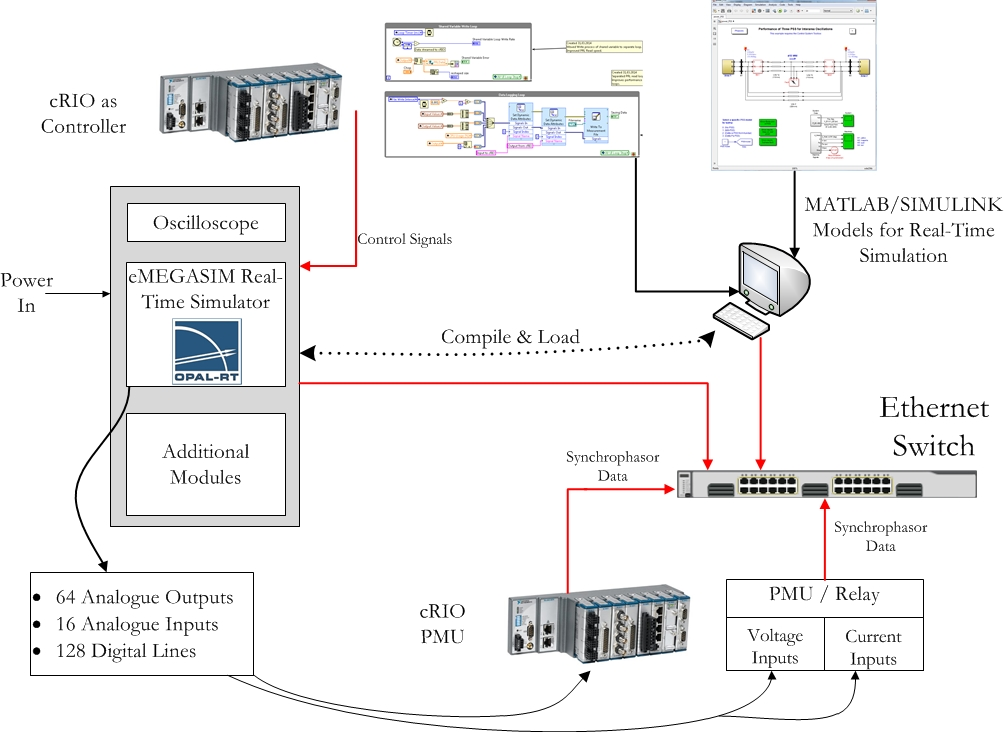
\includegraphics[width=1\linewidth]{./SmarTSlabOutline}
%\caption{Outline of SmarTS Lab at KTH}
%\label{fig:SmarTSlabOutline}
%\end{figure*}

%Appendix two text goes here.


% use section* for acknowledgement
%\section*{Acknowledgment}
%M.S. Almas is supported by the STRON$g^{2}$rid project, funded by Nordic Energy Research.
%L. Vanfretti is supported in part by the STRON$g^{2}$rid project, funded by Nordic Energy Research, in part by the STandUP for Energy collaboration initiative and also by the KTH School of Electrical Engineering.

% Can use something like this to put references on a page
% by themselves when using endfloat and the captionsoff option.
\ifCLASSOPTIONcaptionsoff
  \newpage
\fi



% trigger a \newpage just before the given reference
% number - used to balance the columns on the last page
% adjust value as needed - may need to be readjusted if
% the document is modified later
%\IEEEtriggeratref{8}
% The "triggered" command can be changed if desired:
%\IEEEtriggercmd{\enlargethispage{-5in}}

% references section

% can use a bibliography generated by BibTeX as a .bbl file
% BibTeX documentation can be easily obtained at:
% http://www.ctan.org/tex-archive/biblio/bibtex/contrib/doc/
% The IEEEtran BibTeX style support page is at:
% http://www.michaelshell.org/tex/ieeetran/bibtex/
%\bibliographystyle{IEEEtran}
% argument is your BibTeX string definitions and bibliography database(s)
%\bibliography{IEEEabrv,../bib/paper}
%
% <OR> manually copy in the resultant .bbl file
% set second argument of \begin to the number of references
% (used to reserve space for the reference number labels box)
\begin{thebibliography}{1}

\bibitem{KundurTwoArea} 
M.~Klein, J. G.~Rogers and P.~Kundur \emph{A fundamental study of inter-area oscillations in Power Systems}  IEEE Transactions on Power Systems, Volume. 6, Issue 3, pp. 914-921, 1991. 

\bibitem{WAPODNorway} Kjetil Uhlen, Luigi Vanfretti, MM De Oliveira, AB Leirbukt, Vemund Halmo Aarstrand, Jan O Gjerde \emph{Wide-Area Power Oscillation Damper implementation and testing in the Norwegian transmission network} in Power and Energy Society General Meeting, 2012 IEEE pp. 1-7

\bibitem{localREMcomparison}  M. E.~Aboul-Ela, A. A.~Sallam, J. D.~McCalley and A. A.~Fouad, \emph{Damping Controller Design for Power System Oscillations Using Global Signals}, IEEE trans. on Power Systems, Vol. 11, No. 2, May 1996, pp. 767-773

\bibitem{Yuwa}  Luigi Vanfretti, Yuwa Chompoobutrgool, Joe H Chow, \emph{Chapter 10: Inter-Area Mode Analysis for Large Power Systems using Synchrophasor Data}, Book Chapter, in Coherency and Model Reduction of Large Power Systems, Joe H. Chow (Ed.), Springer, 2013.

\bibitem{Rogers_book} G.~Rogers \emph{Power system oscillations}, Springer Science \& Business Media, 2012. 

\bibitem{WAPODChina} Li Peng and Wu Xiaochen and Lu Chao and Shi Jinghai and Hu Jiong and He Jingbo and Zhao Yong and Aidong Xu \emph{Implementation of CSG's Wide-Area Damping Control System: Overview and experience} in Power Systems Conference and Exposition, 2009. PSCE '09. IEEE/PES pp. 1-9

\bibitem{China_paper} Zhang, F., Sun, Y., Cheng, L., Li, X., Chow, J. H., \& Zhao, W. (2015) \emph{Measurement and modeling of delays in wide-area closed-loop control systems} IEEE Transactions on Power Systems, 30(5), 2426-2433.

\bibitem{Biplab} Pal, S., Sikdar, B. and Chow, J.H., 2018. \emph{An online mechanism for detection of gray-hole attacks on PMU data} IEEE Transactions on Smart Grid, 9(4), pp.2498-2507.

\bibitem{Kamwa} Grondin, R., I. Kamwa, G. Trudel, L. Gerin-Lajoie, and J. Taborda. "Modeling and closed-loop validation of a new PSS concept, the multi-band PSS." In Power Engineering Society General Meeting, 2003, IEEE, vol. 3, pp. 1804-1809. IEEE, 2003.

%\bibitem{CommDelay} CFM Danielson, Luigi Vanfretti, Muhammad Shoaib Almas, Y Choompoobutrgool, JO Gjerde \emph{Analysis of communication network challenges for synchrophasor-based wide-area applications} Bulk Power System Dynamics and Control - IX Optimization, Security and Control of the Emerging Power Grid (IREP), 2013 IREP Symposium pp 1-13

%\bibitem{YuwaDelay} Yuwa Chompoobutrgool, Luigi Vanfretti \emph{Analysis of time delay effects for wide-area damping control design using dominant path signals}, PES General Meeting| Conference \& Exposition, 2014 IEEE, pp 1-5

\bibitem{PhasorPOD} 
L.~\"{A}ngquist and C.~Gama  \emph{Damping Algorithm based on Phasor Estimation} in Power Engineering Society Winter Meeting, 2001. IEEE, Volume 3, pp. 1160 - 1165  

\bibitem{eMEGASIM} \emph{eMEGASIM Power Grid Real-Time Digital Hardware in the Loop Simulator} Available Online at : \url{http://www.opal-rt.com/}

%\bibitem{Dmello} F. P.~Dmello, and. \ C.~Concordia
%\emph{Concepts of Synchronous Machine Stability as Affected by Excitation Control} IEEE TRANSACTIONS ON POWER APPARATUS AND SYSTEMS, vol. PAS 88, no. 4, 1969. 
  


\bibitem{WAMTCSC} J.C~Agee , S~Patterson, R~Beaulieu, Coultes \ M.,Grondin \ R. , Kamwa \ I.,
Trudel \ G., Godhwani \ A. , Bérubé \ R. , Hajagos \ L. , Malik \ O. , Murdoch \ A.,Boukarim \ G. , Taborda \ J. , and Thornton-Jones \ R. \emph{IEEE tutorial course in Power System stabilization via excitation control.} Technical report, June 2007


\bibitem{TaskForce} M.Crow, M. Gibbard, A. Messina, J. Pierre, J. Sanchez-Gasca, D. Trudnowski, D. Vowles \emph{Identification of Electromechanical Modes in Power Systems} IEEE Task Force Report, Special Publication TP462, June 2012.

\bibitem{Chaudhuri} N.S.~Chaudhuri, R.~Majumder and B~ Chaudhuri \emph{Interaction between conventional and adaptive phasor power oscillation damping controllers} in Power and Energy Society General Meeting, 2010 IEEE Minneapolis, MN, 2012 pp. 1-7
  
\bibitem{PhasorPODImplement} M.~Shoaib Almas and L.~Vanfretti, \emph{Implementation of Conventional PSS and Phasor Based POD for Power Stabilizing Controls for Real-Time Simulation}, IEEE IES IECON14, 29 Oct-1 Nov, 2014, Dallas, USA.
%\bibitem{OPALemegasim} eMEGAsim PowerGrid Real-Time Digital Hardware in the Loop Simulator — Opal RT, [Online]. Available: \url{http://www.opal-rt.com/}

\bibitem{cRIO9081} \emph{Operating Instructions and Specifications Compact RIO NI cRIO-9081/9082 and cRIO-9075/9076}, National Instruments, Available Online at \url{http://www.ni.com/pdf/manuals/}

%\bibitem{SDK} Luigi Vanfretti, Vemund H Aarstrand, M Shoaib Almas, Vedran S Peric, Jan O Gjerde, \emph{A Software Development Toolkit for Real-Time Synchrophasor Applications},  IEEE PES Grenoble PowerTech, 2013, DOI: 10.1109/PTC.2013.6652191

\bibitem{Rebello_WAPOD_Software}Eldrich Rebello, Luigi Vanfretti, and Md Shoaib Almas. \emph{Software architecture development and implementation of a synchrophasor-based real-time oscillation damping control system} In PowerTech, 2015 IEEE Eindhoven, pp. 1-6. IEEE, 2015.

\bibitem{SmarTSLab} M.S. Almas, M. Baudette, L. Vanfretti, S. Lovlund and J.O. Gjerde "\emph{Synchrophasor network, laboratory and software applications developed in the STRON$g^{2}$rid project}," PES General Meeting, Conference Exposition, July 2014 IEEE pp 1 - 5

\bibitem{sVARdamp} E.V~Larsen and E.H~Chow, General Electric Company, NY, \emph{Application of Static VAR Systems for System Dynamic Performance}, 1987 IEEE pp. 43-46






  
%\bibitem{cRIO9076} \emph{Operating Instructions and Specifications Compact RIO NI cRIO-9075/9076}, National Instruments, Available Online at \url{http://www.ni.com/pdf/manuals/375650b.pdf}

\bibitem{LabviewTemplate} \emph{FPGA Control on Compact RIO Sample Project Documentation}, National Instruments, Available Online at \url{http://www.ni.com/white-paper/14137/en/}


\bibitem{MATLABexample} Grondin, R., Kamwa, I., Trudel, G., Gerin-Lajoie, L. and Taborda, J., 2003, July. \emph{Modeling and closed-loop validation of a new PSS concept, the multi-band PSS} In Power Engineering Society General Meeting, 2003, IEEE (Vol. 3, pp. 1804-1809). IEEE.

\bibitem{PSSDocumentation} \emph{Generic Power System Stabilizer} Documentation distributed with \textsc{Matlab} R2014a Available online at \url{http://www.mathworks.se/help/physmod/sps/powersys/ref/genericpowersystemstabilizer.html}

\bibitem{LabViewManuals} \emph{IP Corner: The LabVIEW Fixed-Point Data Type Part 1 – Fixed-Point 101, Available Online at} \url{http://www.ni.com/newsletter/50303/en/}, Dec 20, 2011 



%\bibitem{BabelFish} Muhammad Shoaib Almas, Luigi Vanfretti, Maxime Baudette, \emph{BabelFish\textendash Tools for IEEE C37. 118.2-compliant real-time synchrophasor data mediation}, SoftwareX Volume 6, 2017, Pages 209-216 \url{https://doi.org/10.1016/j.softx.2017.08.002}

\bibitem{Audur} L Vanfretti, GM J\'{o}nsd\'{o}ttir, MS Almas, E Rebello, SR Firouzi, M Baudette \emph{Audur\textendash A platform for synchrophasor-based power system wide-area control system implementation}, SoftwareX Volume 7, January\textendash June 2018, Pages 294-301 \url{ttps://doi.org/10.1016/j.softx.2018.08.003}


%\bibitem{LabVIEWCourse} \emph{LabVIEW Course Manuals - Core 1, Real Time, FPGA, August 2012 Editions}, Copyright 2012 National Instruments

%\bibitem{NISharedVar} \emph{National Instruments, Sending Shared Variable Data over the Network Immediately} National Instuments,\ P. Web Resource. Online Document. Last Updated June 2011.
%Retreived On 13.03.2014. Available At:  \url{http://zone.ni.com/reference/en-XX/help/371361H-01/lvconcepts/sv_flush/}    

\end{thebibliography}

% biography section
% 
% If you have an EPS/PDF photo (graphicx package needed) extra braces are
% needed around the contents of the optional argument to biography to prevent
% the LaTeX parser from getting confused when it sees the complicated
% \includegraphics command within an optional argument. (You could create
% your own custom macro containing the \includegraphics command to make things
% simpler here.)
%\begin{biography}[{\includegraphics[width=1in,height=1.25in,clip,keepaspectratio]{mshell}}]{Michael Shell}
% or if you just want to reserve a space for a photo:

%\begin{IEEEbiography}[{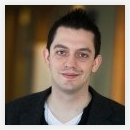
\includegraphics[width=1in,height=1.25in,clip,keepaspectratio]{lvanfretti.PNG}}]{Luigi Vanfretti}
%Luigi Vanfretti (M'10) is an Assistant Professor at the Electric Power Systems Division, School of Electrical Engineering, KTH Royal Institute of Technology, Stockholm, Sweden. He received his M.Sc. and Ph.D. in 2007 and 2009, respectively, both in Electric Power Engineering from Rensselaer Polytechnic Institute, Troy, NY, USA. His main research interest is on the development of PMU data-based applications. Since 2009, he has served as Secretary of the IEEE PES CAMS Task Force on Open Source. He is an evangelist of Free/Libre and Open Source Software.
%\end{IEEEbiography}

%\begin{IEEEbiography}[{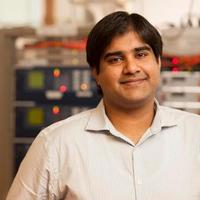
\includegraphics[width=1in,height=1.25in,clip,keepaspectratio]{msalmas.PNG}}]{M S Almas}
%Muhammad Shoaib Almas (Student Member ’12) has received the B.Sc. degree in Electrical Engineering from National University of Sciences and Technology (NUST), Pakistan, in 2007, and the M.Sc. degree in Electric Power Engineering from KTH Royal Institute of Technology, Stockholm, Sweden, in 2011. He is currently a Ph.D. student within the Electric Power Systems (EPS) Division at KTH. The main theme of his current research is the “PMU-assisted real-time distributed control of hybrid AC and DC grids for damping inter-area electromechanical oscillations”. He has a two year professional experience in substation automation and power system protection desgining using microprocessor based protection relays (GE Multilin/GE Energy). His research interests are wide area power system monitoring, protection, automation and control, communication network simulation and cyber security.
%\end{IEEEbiography}

% if you will not have a photo at all:
%\begin{IEEEbiographynophoto}{Eldrich Rebello}
%Eldrich Rebello lives in Springfield and works in Qwik-e-Mart. He is more popularly known as Apu.
%\end{IEEEbiographynophoto}

% insert where needed to balance the two columns on the last page with
% biographies
%\newpage

% You can push biographies down or up by placing
% a \vfill before or after them. The appropriate
% use of \vfill depends on what kind of text is
% on the last page and whether or not the columns
% are being equalized.

%\vfill

% Can be used to pull up biographies so that the bottom of the last one
% is flush with the other column.
%\enlargethispage{-5in}



% that's all folks
\end{document}


